\documentclass[12pt,titlepage]{report}

%polskie znaki
\usepackage[T1]{fontenc}
\usepackage[utf8]{inputenc}
% grafika 
\usepackage[pdftex]{graphicx}
\usepackage{epstopdf}
\usepackage{subfig} 
\usepackage{multicol}
\usepackage{placeins}
%\usepackage{float} - bez tego można ustawić 2 obrazki obok siebie

\usepackage[polish]{babel}
\usepackage{lmodern} %czcionki
\selectlanguage{polish} 
 %zajebiaszcze formatownanie całej strony!
 \usepackage[a4paper,left=1.5cm,right=1.5cm,top=1.5cm,bottom=1.5cm,includefoot=false,includehead=false]{geometry} 
 \usepackage{color} %kolorowy tekst
 
\usepackage[final]{pdfpages}

\title{Przetwarzanie Sygnałów}
\author{Jakub Dudarewicz}
\date{Semestr letni, 2016}

\begin{document}

\begin{titlepage}
	\maketitle
\end{titlepage}
	
%definicja formatowania nagłówków
	\def\thesection{Instrukcja \arabic{section}.\Large}
	\def\thesubsection{Instrukcja \arabic{section}, zadanie \arabic{subsection}\normalsize}
	\def\theparagraph{\normalsize}%doesnotwork
\section{Podstawy generacji sygnałów}
\subsection{Operacje tablicowe i macierzowe}

Wynik operacji mnożenia macierzowego i tablicowego:
\begin{multicols}{2}
	{
		\small
		\begin{verbatim}
		A =		
		1   43   45
		
		B =		
		6   12   45
		2    4   56
		12    3    1
		
		tablicowe
		6    516   2025
		2    172   2520
		12    129     45
		
		macierzowe
		632    319   2498
		\end{verbatim}
	}
\end{multicols}
Operacje te są fundamentalnie od siebie różne

\subsection{Próbkowanie przebiegu sinusoidalnego}
M-plik użyty do generacji wykresów:
\begin{multicols}{3}
	{
		\tiny
		\begin{verbatim}
		% probkowanie sinusa
		
		n=10; %długość obserwacji
		k=100; %liczba próbek
		t=[1:k];
		
		H = figure;
		
		m=500;
		a=sin(2*pi*n*t/m);
		subplot(221);
		plot(a);
		title("500");
		
		m=200;
		a=sin(2*pi*n*(t/m));
		subplot(222);
		plot(a);
		title("200");
		
		m=100;
		a=sin(2*pi*n*t/m);
		subplot(223);
		plot(a);
		title("100");
		
		m=20;
		a=sin(2*pi*n*t/m);
		subplot(224);
		plot(a);
		title("20");
		
		clear;
		\end{verbatim}
	}
\end{multicols}
\begin{figure}[!h]
	\centering
	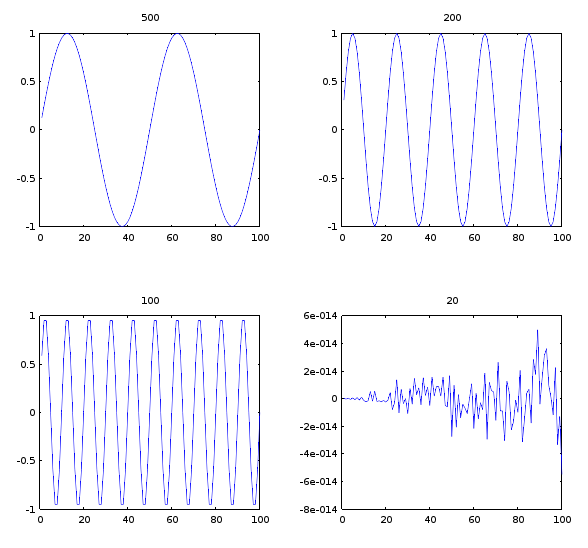
\includegraphics[scale=0.7]{../cw03_output}
	\caption{Przebieg sinusoidalny próbkowany z różnymi częstotliwościami}
\end{figure}
Liczba zarejestrowanych okresów i rozdzielczość wynika z częstotliwości próbkowania. W tym zadaniu nie przekształcam dziedziny sygnału do czasu.
\newpage

\subsection{Skok jednostkowy}

M-plik użty do genracji wykresów:
\begin{multicols}{3}
	{
		\tiny
		\begin{verbatim}
		%skok jednostkowy
		
		be = 10;
		en = 30;
		dur = 100;
		
		a = zeros(dur,1);
		
		for i = be:en
		a(be, 1) = 1;
		be = be + 1;
		end
		
		figure;
		plot(a);
		axis([0, 100, -0.5, 1.5]);
		title("skok jednostkowy");
		\end{verbatim}
	}
\end{multicols}

\begin{figure}[!h]
	\centering
	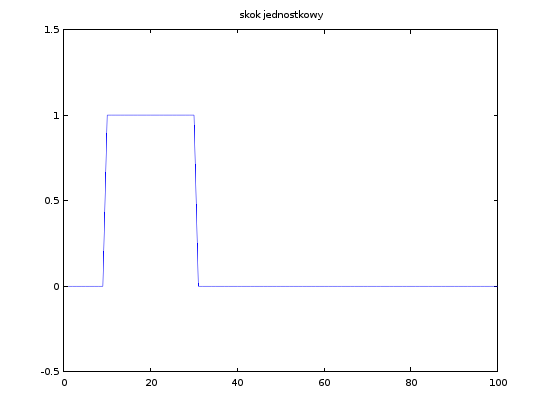
\includegraphics[scale=0.5]{../cw04_output}
	\caption{Przykładowy wydruk skoku jednostkowego}
\end{figure}

\subsection{Skok jednostkowy, użycie varargin}
M-plik użyty do generowania wykresów:
\begin{multicols}{3}
	{
		\tiny
		\begin{verbatim}
		function skok(varargin) %(duration,
		begin 1, end 1, begin 2, end 2...
		
		k = 2;
		l=1;
		figure;
		r = ceil((nargin-1)/4);
		dur = varargin{1};
		
		for i = 1:((nargin-1)/2)
		be = varargin{k};
		en = varargin{k+1};
		
		
		a = zeros(dur,1);
		
		for j = be:en
		a(be, 1) = 1;
		be += 1;
		end
		
		subplot(r, 2, l);
		plot(a, '.');
		axis([0, dur, -0.5, 1.5]);
		printf("bound %d - %d\n", varargin{k},
		varargin{k+1});
		
		if(k+1<(nargin-1))
		k=k+2;
		endif
		l=l+1;
		end
		
		endfunction
		\end{verbatim}
	}
\end{multicols}

\begin{figure}[!h]
	\centering
	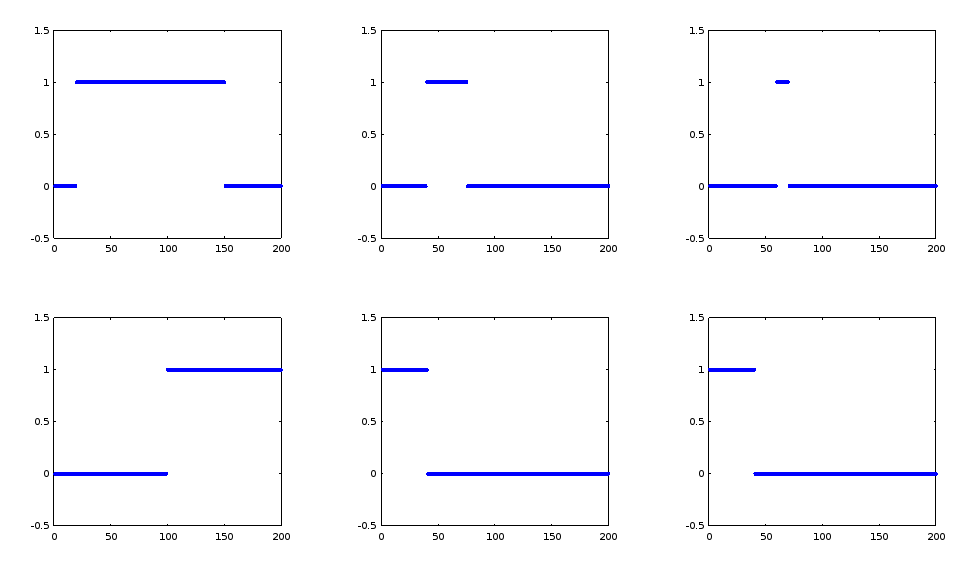
\includegraphics[scale=0.5]{../cw05_output}
	\caption{Przykładowy wydruk dla siedmiu argumentów}
\end{figure}
Funkcja varargin i wszystkie jej towarzyszące są bardzo użyteczne, bo pozwalają na napisanie bardziej uniwersalnej funkcji.
\newpage

\subsection{Przebieg wykładniczy zespolony}
M-plik użyty do generacji wykresów funkcji $f\left(x\right)={e}^{xi}$:
\begin{multicols}{3}
	{
		\tiny
		\begin{verbatim}
		%przebieg wykładniczy zespolony
		
		t=[0:0.1:2*pi];
		
		zesp=e.^(t.*j);
		rzecz=real(zesp);
		uroj=imag(zesp);
		modul=abs(zesp);
		faza=angle(zesp);
		
		figure
		
		subplot(121)
		plot(zesp)
		title("plaszczyzna zespolona")
		subplot(243)
		plot(modul)
		title("modul")
		subplot(244)
		plot(rzecz)
		title("skladnik rzeczywisty")
		subplot(247)
		plot(uroj)
		title("skladnik urojony")
		subplot(248)
		plot(faza)
		title("kat fazowy")
		\end{verbatim}
	}
\end{multicols}

\begin{figure}[!h]
	\centering
	\subfloat[$0i - \pi i$]{
		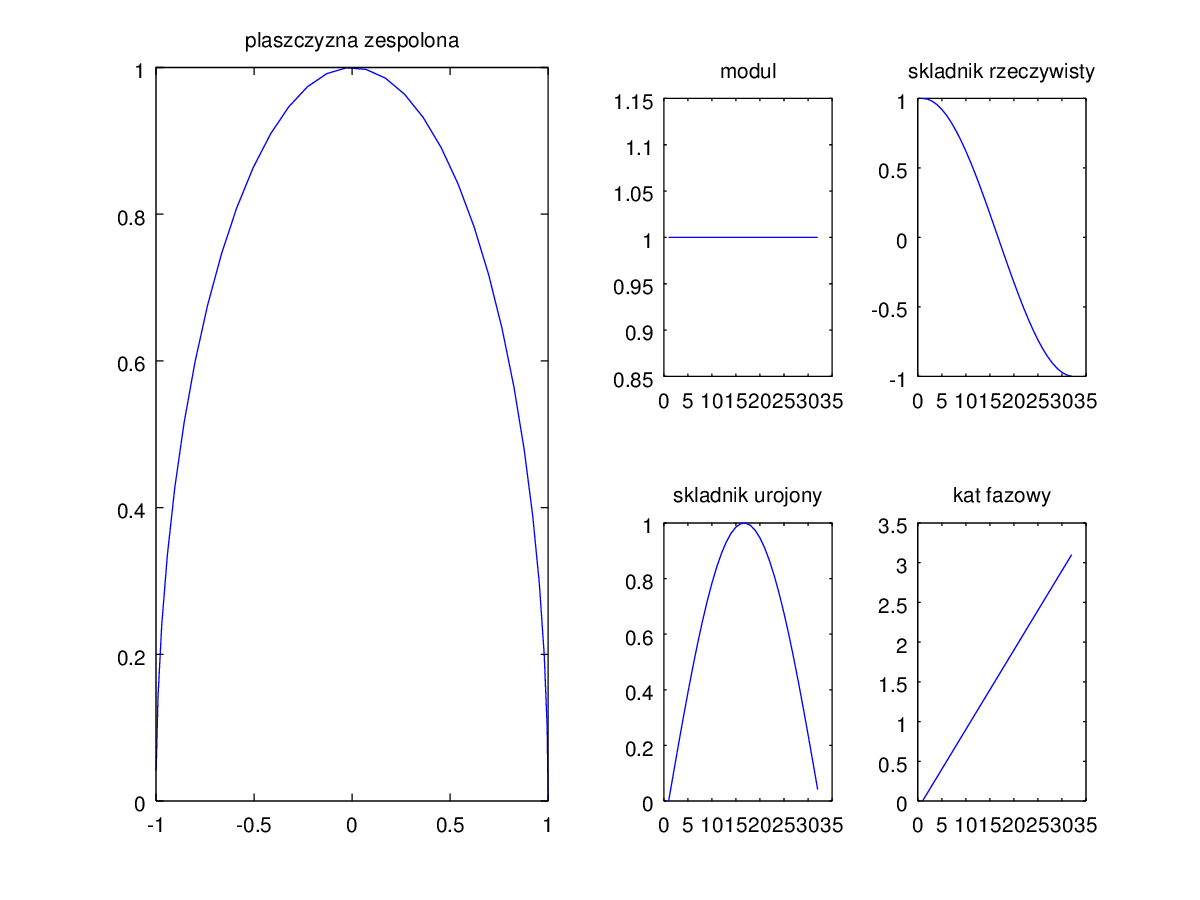
\includegraphics[scale=0.5]{../cw06_output}
	}
	\par
	\subfloat[$0i - 2\pi i$]{
		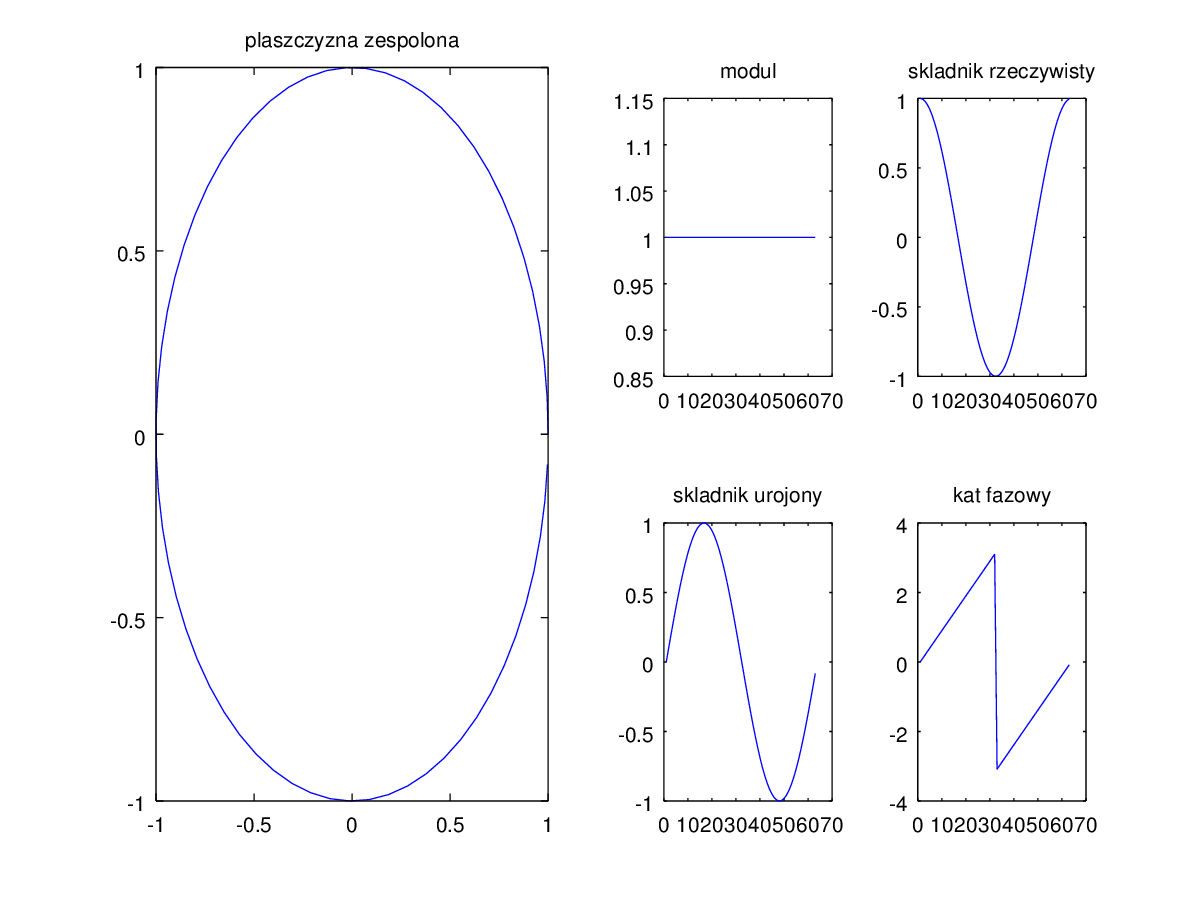
\includegraphics[scale=0.5]{../cw06_output_2pi}
	}
	\caption{Zespolone przebiegi wykładnicze dla dwóch zakresów zmiennej zespolonej}
\end{figure}
Z powyższych wykresów połączenie funkcji wykładniczej zespolonej z funkcjami trygonometrycznymi jest oczywiste. Zrozumiała też staje się słynna Tożsamość Eulera ${e}^{\pi i} + 1 = 0$.
\newpage

\subsection{Modulowanie przebiegu sinusoidalnego}
M-plik użyty do generacji wykresów:
\begin{multicols}{2}
	{
		\tiny
		\begin{verbatim}
		%modulowanie sinusa
		
		n=1; %długość obserwacji
		k=1000; %liczba próbek
		t=[1:k]; %probki
		m=500; %czestotliwosc obserwacji
		
		a=sin(2*pi*n*t/m);
		b=(0.5).*sin((10*2*pi*n*t/m)+pi);
		
		c=a.*b;
		
		figure
		
		subplot(121)
		plot(c)
		subplot(222)
		plot(a)
		subplot(224)
		plot(b)
		\end{verbatim}
	}
\end{multicols}

\begin{figure}[!h]
	\centering
	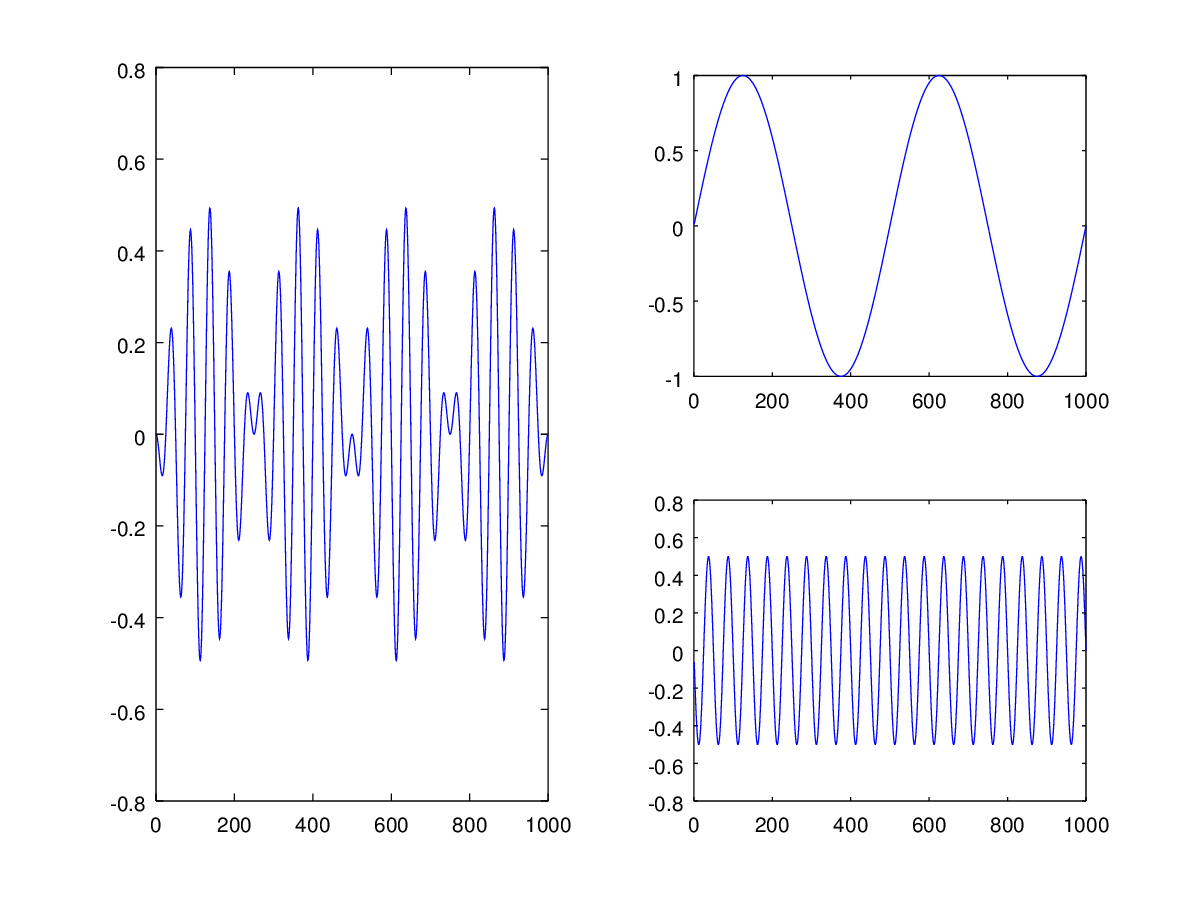
\includegraphics[scale=0.4]{../cw07_output}
	\caption{Z lewej - sygnał zmodulowany, z prawej - sygnały wyjściowe}
\end{figure}
Modulacja osiągana jest poprzez pomnożenie tablicowe przez siebie dwóch sygnałów.
\newpage

\section{Podstawy próbkowania sygnałów}
\subsection{Generowanie przebiegów sinusoidalnych o pulsacji znormalizowanej}
M-plik użyty do generacji wykresów:
\begin{multicols}{2}
	{
		\tiny
		\begin{verbatim}
		n=[0:127];
		
		xa=sin((pi/20)*n);
		xb=sin((pi/4)*n);
		xc=sin((pi/2)*n);
		xd=sin((pi/2+2*pi)*n);
		xe=sin((pi/2+0.01)*n);
		
		subplot(131)
		stem(xa)
		title('\pi/20')
		subplot(232)
		stem(xb)
		title('\pi/4')
		subplot(233)
		stem(xc)
		title('\pi/2')
		subplot(235)
		stem(xd)
		title('\pi/20 + 2\pi')
		subplot(236)
		stem(xe)
		title('\pi/20 + 0.01')
		\end{verbatim}
	}
\end{multicols}
\begin{figure}[!h]
	\centering
	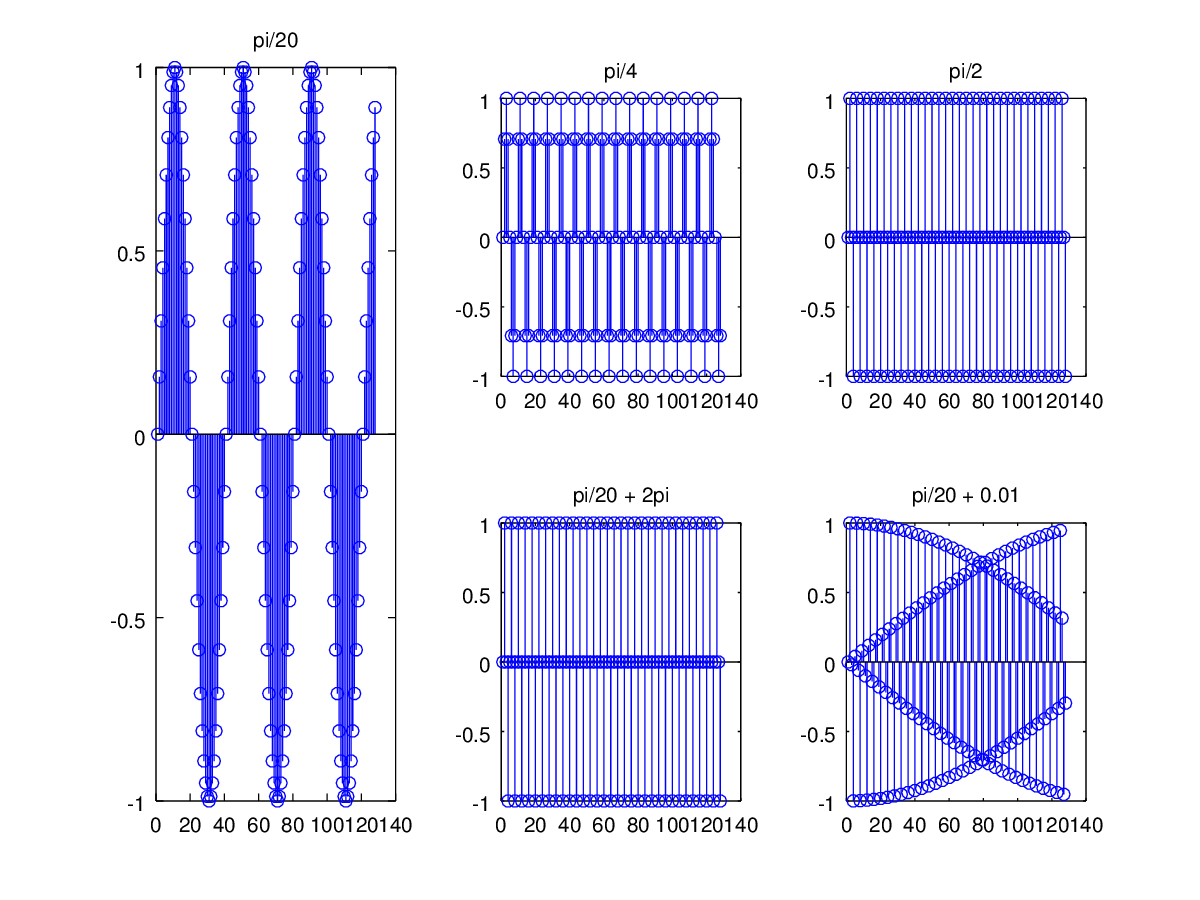
\includegraphics[scale=0.7]{../cw11_output}
	\caption{Przebiegi generowane dla różnych pulsacji.}
\end{figure}
Zbyt duża częstotliwość powoduje niedokładne rejestrowanie przebiegu.
\newpage

\subsection{Generowanie przebiegów sinusoidalnych próbkowanych z różną częstotliwością}
M-plik użyty do generacji wykresów:
\begin{multicols}{3}
	{
		\tiny
		\begin{verbatim}
		%sampling frequency
		fsa=4000;
		fsb=4020;
		fsc=8000;
		fsd=19000;
		fse=44000;
		
		%samples vector
		n=[0:127];
		
		%signal frequency
		f=2000;
		
		%time vectors
		ta=n/fsa;
		tb=n/fsb;
		tc=n/fsc;
		td=n/fsd;
		te=n/fse;
		
		
		%signal model
		xa=sin(2*pi*f*ta);
		xb=sin(2*pi*f*tb);
		xc=sin(2*pi*f*tc);
		xd=sin(2*pi*f*td);
		xe=sin(2*pi*f*te);
		
		subplot(131)
		stem(ta, xa)
		title('sampling rate 4000Hz')
		subplot(232)
		stem(tb, xb)
		title('sampling rate 4020Hz')
		subplot(233)
		stem(tc, xc)
		title('sampling rate 8000Hz')
		subplot(235)
		stem(td, xd)
		title('sampling rate 19000Hz')
		subplot(236)
		stem(te, xe)
		title('sampling rate 44000Hz')
		\end{verbatim}
	}
\end{multicols}
\begin{figure}[!h]
	\centering
	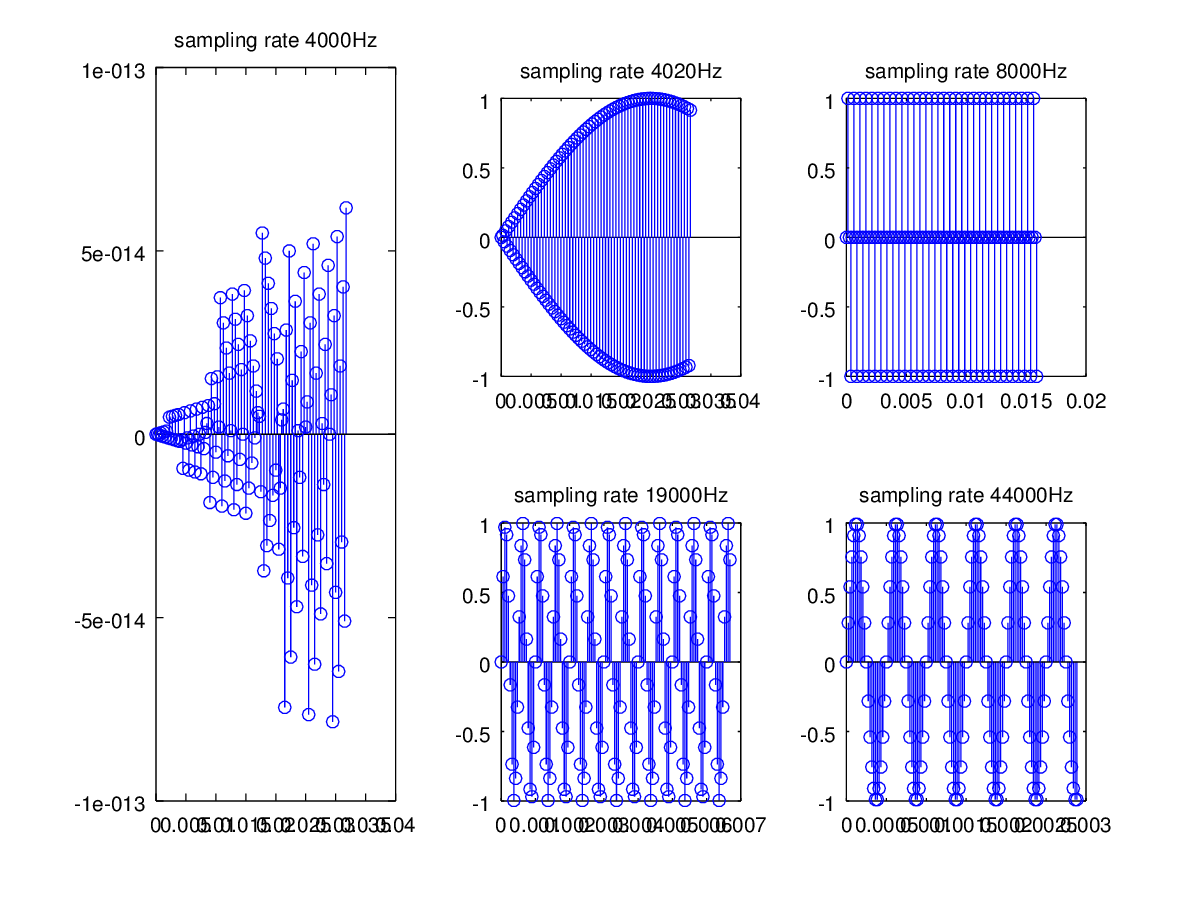
\includegraphics[scale=0.7]{../cw12_output}
	\caption{Przebiegi o równej częstotliwości próbkowane z różną częstotliwością wyświetlone w dziedzinie czasu}
\end{figure}
\newpage

\subsection{Generowanie przebiegów sinusoidalnych przesuniętych w fazie}
M-plik użyty do generacji wykresów:
\begin{multicols}{3}
	{
		\tiny
		\begin{verbatim}
		%sampling frequency
		fs=4000;
		
		%samples vector
		n=[0:63];
		
		%signal frequency
		f=2000;
		
		%time vectors
		t=n/fs;
		
		%signal model
		xa=sin(2*pi*f*t);
		xb=sin(2*pi*f*t + pi/4);
		xc=sin(2*pi*f*t + pi/2);
		xd=sin(2*pi*f*t + 0.11*pi);
		
		subplot(221)
		stem(t, xa)
		title('\phi_1 = 0', 'fontsize', 15)
		subplot(222)
		stem(t, xb)
		title('\phi_1 = \pi/4', 'fontsize', 15)
		subplot(223)
		stem(t, xc)
		title('\phi_1 = \pi/2', 'fontsize', 15)
		subplot(224)
		stem(t, xd)
		title('\phi_1 = 0.11\pi', 'fontsize', 15)
		\end{verbatim}
	}
\end{multicols}
\begin{figure}[!h]
	\centering
	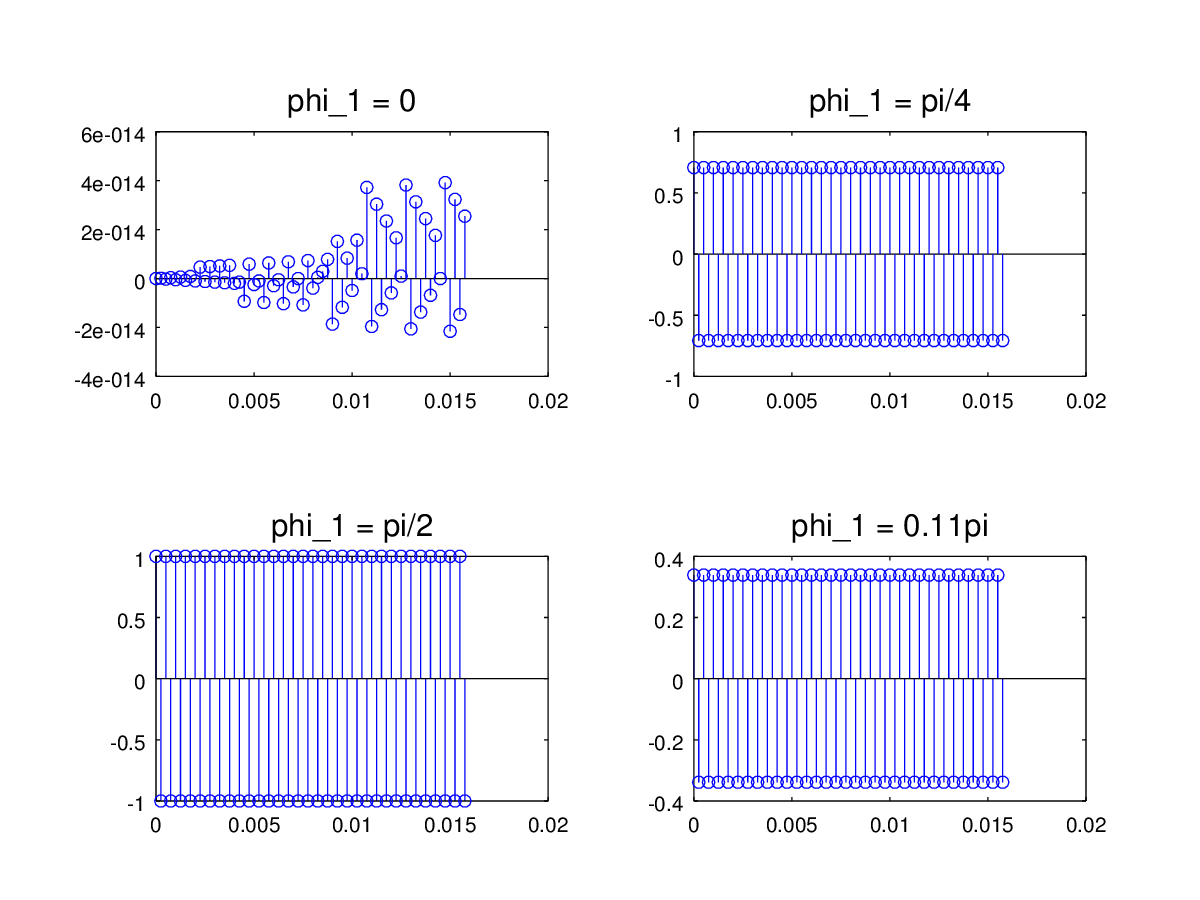
\includegraphics[scale=0.7]{../cw13_output}
	\caption{Przebiegi o równej częstotliwości z różnym przesunięciem fazowym i próbkowane z równą częstotliwością}
\end{figure}
Ponieważ częstotliwość próbkowania sygnału jest dwukrotnie większa od częstotliwości sygnału sygnał jest próbkowany zawsze w tych samych dwóch miejscach w okresie. Od przesunięcia fazowego sygnału zależy jakie wielkości osiągną próbki.
\newpage

\subsection{Generowanie przebiegów sinusoidalnych o rożnych częstotliwościach}
M-plik użyty do generacji wykresów:
\begin{multicols}{3}
	{
		\tiny
		\begin{verbatim}
		%sampling frequency
		fs=4000;
		
		%samples vector
		n=[0:127];
		
		%signal frequency
		fa=1800;
		fb=2200;
		fc=5800;
		
		%time vectors
		t=n/fs;
		
		%signal model
		xa=sin(2*pi*fa*t);
		xb=sin(2*pi*fb*t);
		xc=sin(2*pi*fc*t);
		
		subplot(311)
		stem(t, xa)
		title('f = 1800Hz', 'fontsize', 15)
		subplot(312)
		stem(t, xb)
		title('f = 2200Hz', 'fontsize', 15)
		subplot(313)
		stem(t, xc)
		title('f = 5800Hz', 'fontsize', 15)
		\end{verbatim}
	}
\end{multicols}
\begin{figure}[!h]
	\centering
	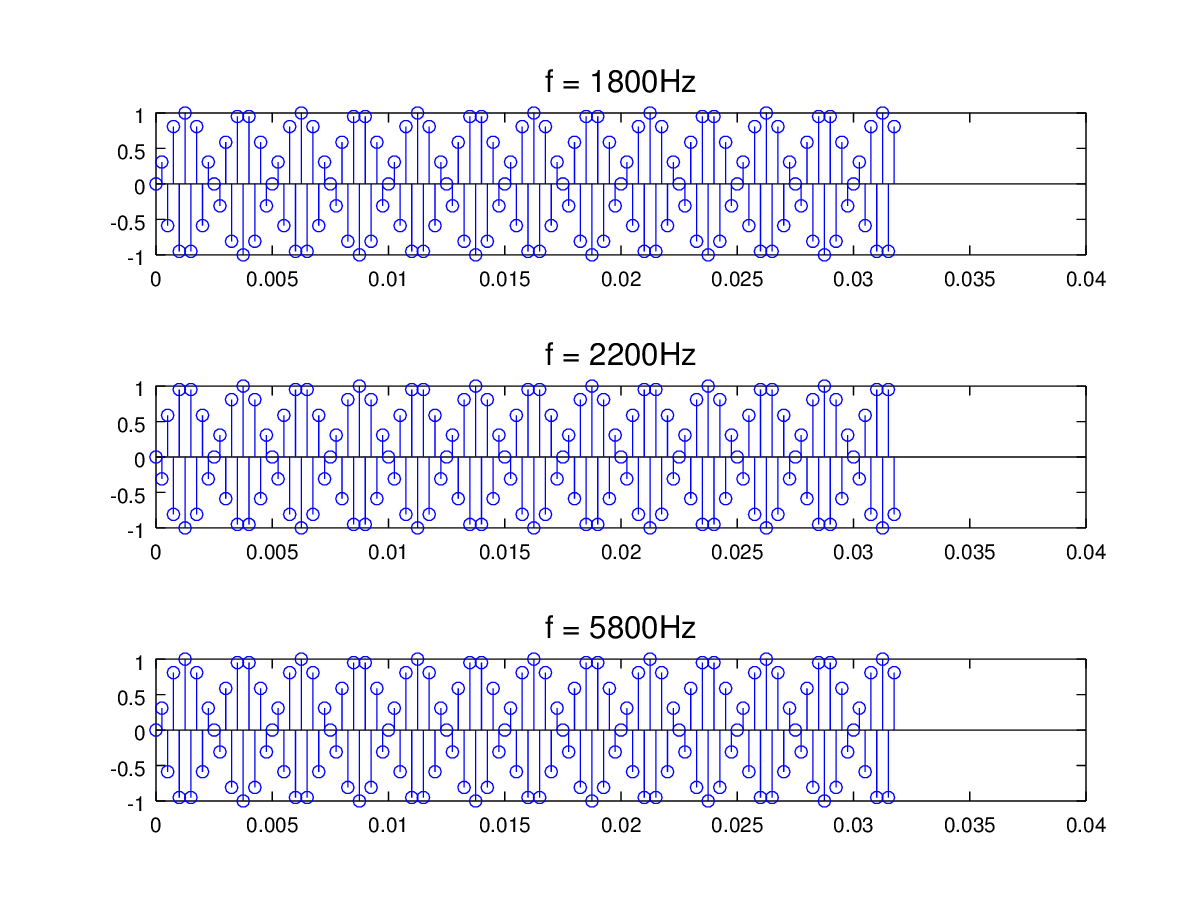
\includegraphics[scale=0.7]{../cw14_output}
	\caption{Przebiegi o różnej częstotliwości próbkowane z równą częstotliwością wyświetlone w dziedzinie czasu}
\end{figure}
\newpage

\subsection{Rekonstrukcja sygnałów cyfrowych}
M-plik użyty do generacji wykresów:
\begin{multicols}{3}
	{
		\tiny
		\begin{verbatim}
		%sampling frequency
		fsa=44000;
		fsd=1000;
		
		%samples vector
		nd=[0:15];
		na=[0:44*length(nd)];
		
		%signal frequency
		f=100;
		
		%time vectors
		ta=na/fsa;
		td=nd/fsd;
		
		%signal model
		xa=sin(2*pi*f*ta);
		xd=sin(2*pi*f*td);
		
		%reconstructions
		xl=interp1(td, xd, ta, "linear");
		xn=interp1(td, xd, ta, "nearest");
		
		xs=zeros(size(ta));
		for  k = 1:length(td);
		st = xd(k)*sinc(fsd*(ta-td(k)));
		xs = xs + st;
		end
		
		hold on
		
		subplot(222)
		plot(ta, xs, 'r')
		hold on
		plot(ta, xa)
		title("sygnal odtworzony interpolacja sinc"
		, "fontsize", 12)
		
		subplot(223)
		plot(ta, xl)
		title("sygnal odtworzony interpolacja linear"
		, "fontsize", 12)
		
		subplot(224)
		plot(ta, xn)
		title("sygnal odtworzony interpolacja nearest"
		, "fontsize", 12)
		
		subplot(221)
		stem(td, xd)
		hold on
		plot(ta, xa)
		title("sygnal analogowy i sprobkowany"
		, "fontsize", 12)
		\end{verbatim}
	}
\end{multicols}
\begin{figure}[!h]
	\centering
	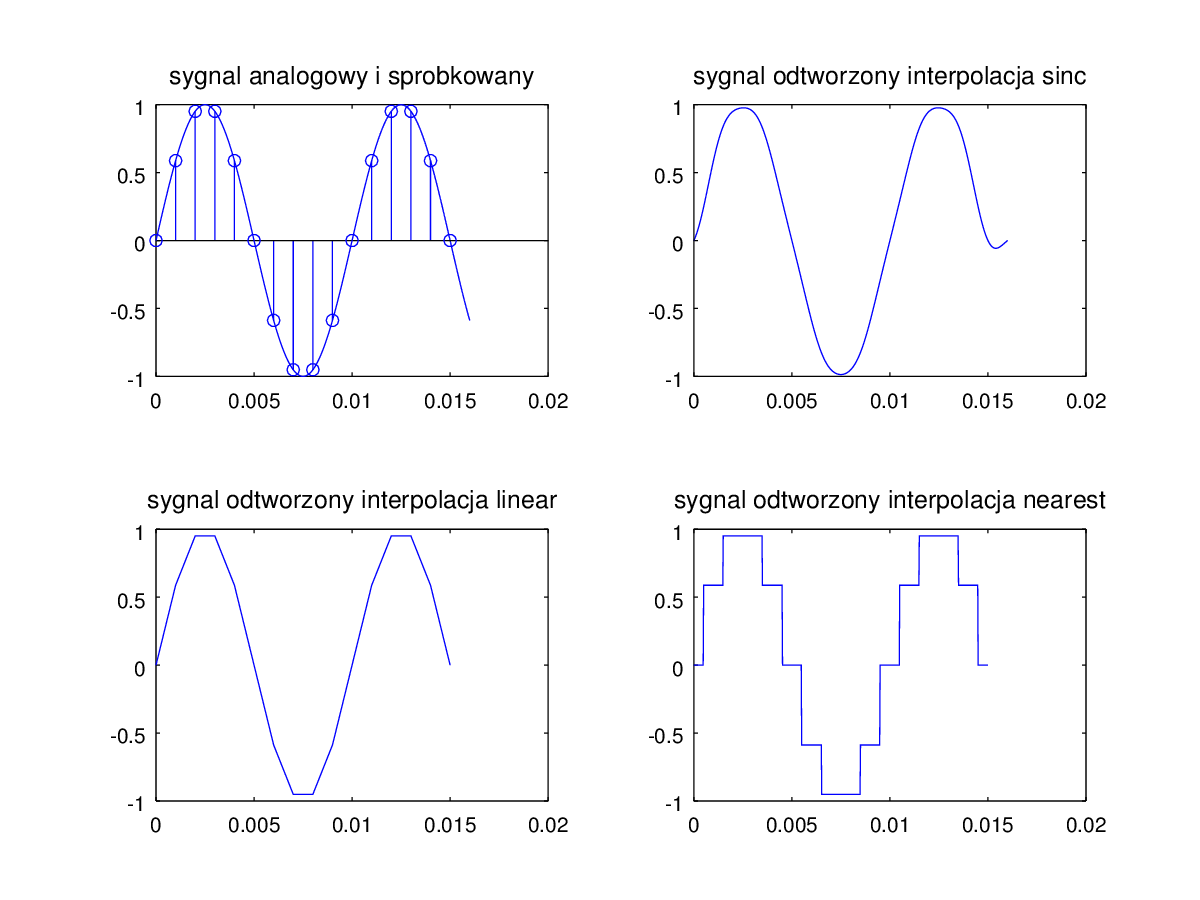
\includegraphics[scale=0.7]{../cw15_output}
	\caption{Sygnały zrekonstruowane za pomocą trzech algorytmów}
\end{figure}
Z wybranych algorytmów najbliżej oryginalnego jest przybliżenie za pomocą funkcji sinc. Interpolacja typu linear wprowadza dużo składowych o wysokiej częstotliwości. natomiast interpolacja nearest nie nadaje się w zasadzie do niczego.
\newpage

\section{Transformata Fourriera}
\subsection{Podstawy DFT} 
\begin{figure}
	\centering
	\subfloat[]{
		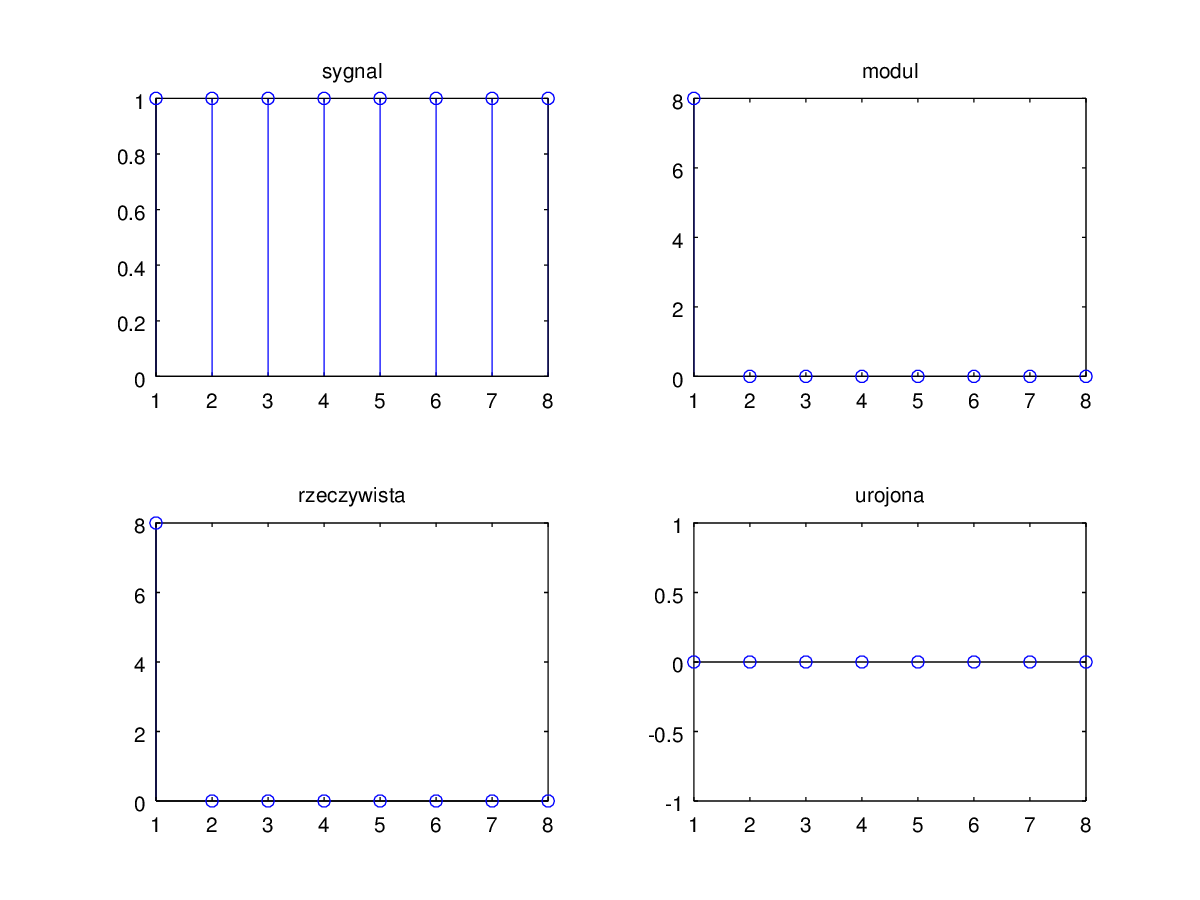
\includegraphics[scale=0.45]{../cw21_output_a}
	}
	\subfloat[]{
		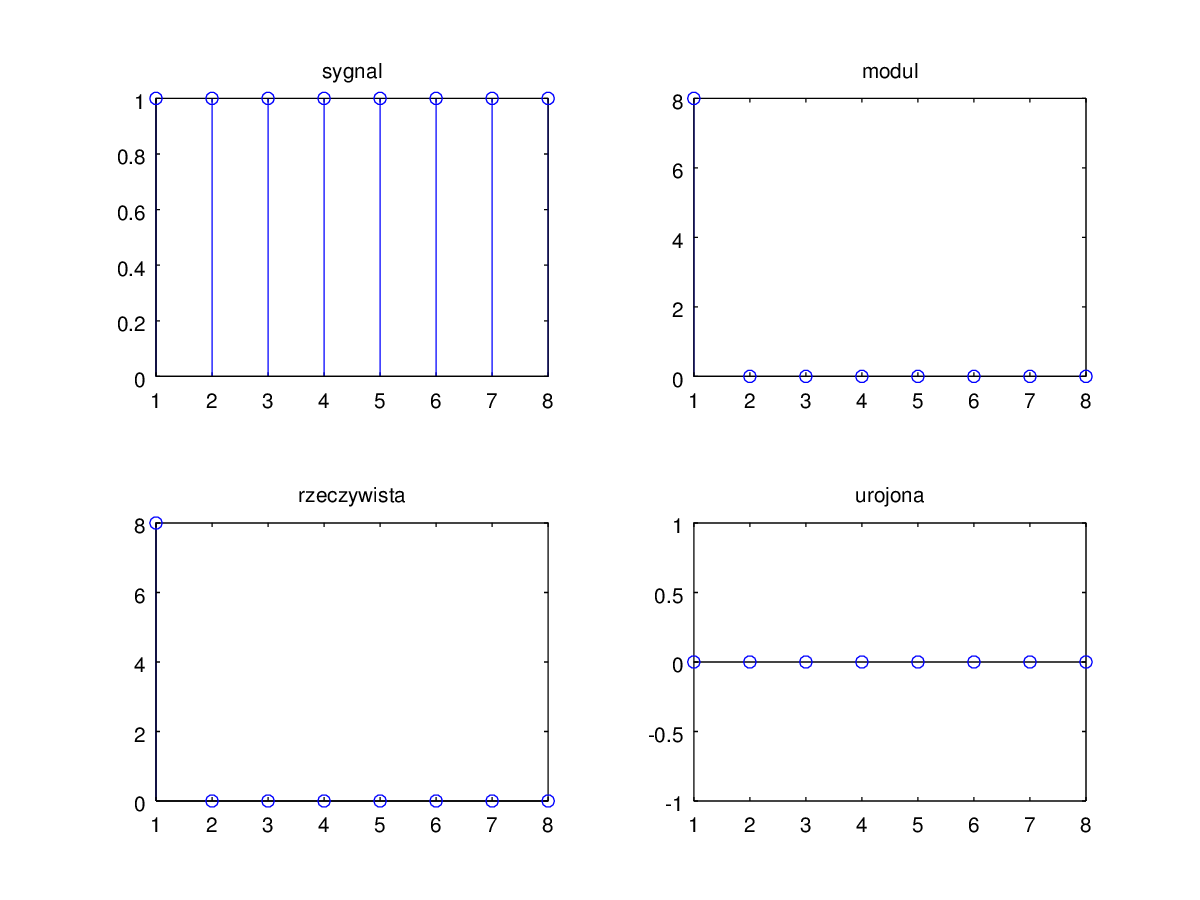
\includegraphics[scale=0.45]{../cw21_output_b}
	}
	\par
	\subfloat[]{
		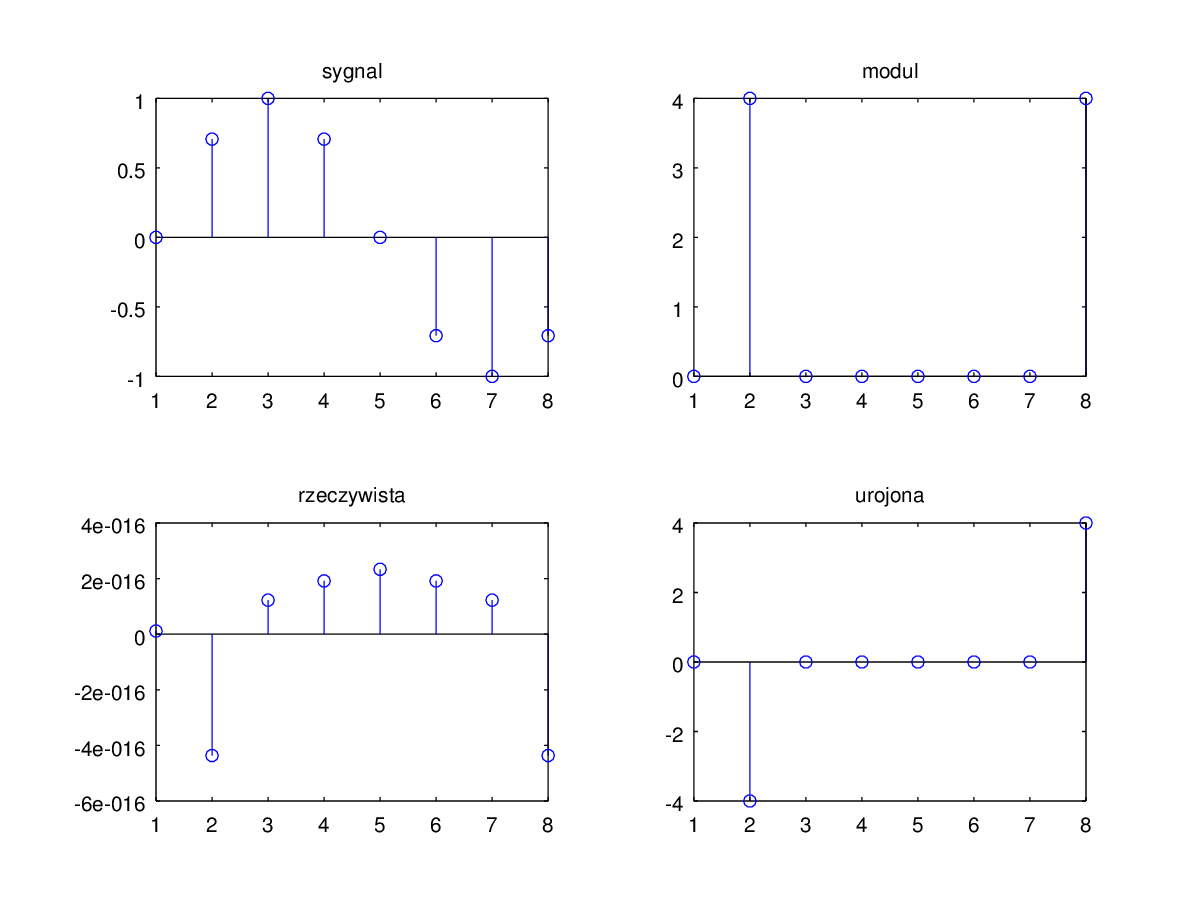
\includegraphics[scale=0.45]{../cw21_output_c}
	}
	\subfloat[]{
		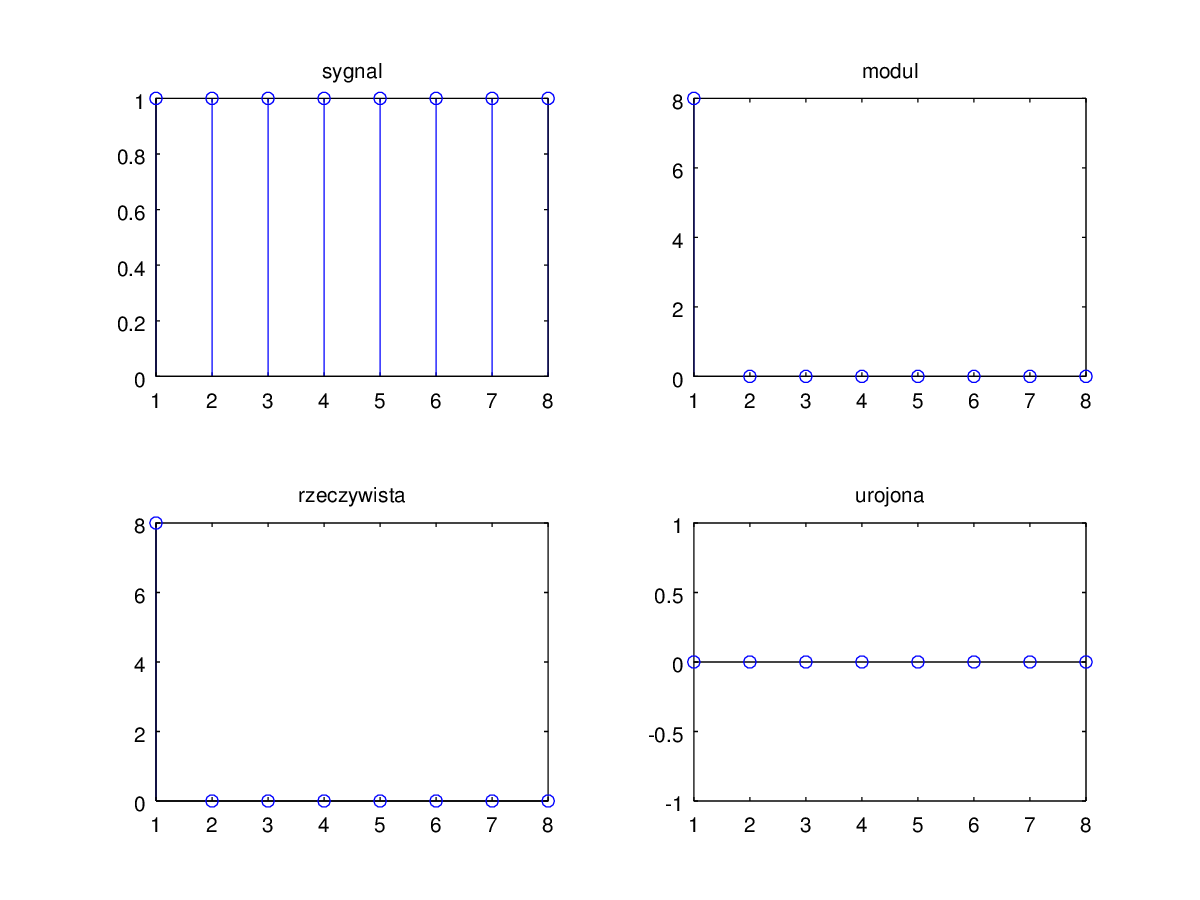
\includegraphics[scale=0.45]{../cw21_output_d}
	}
	\par
	\subfloat[]{
		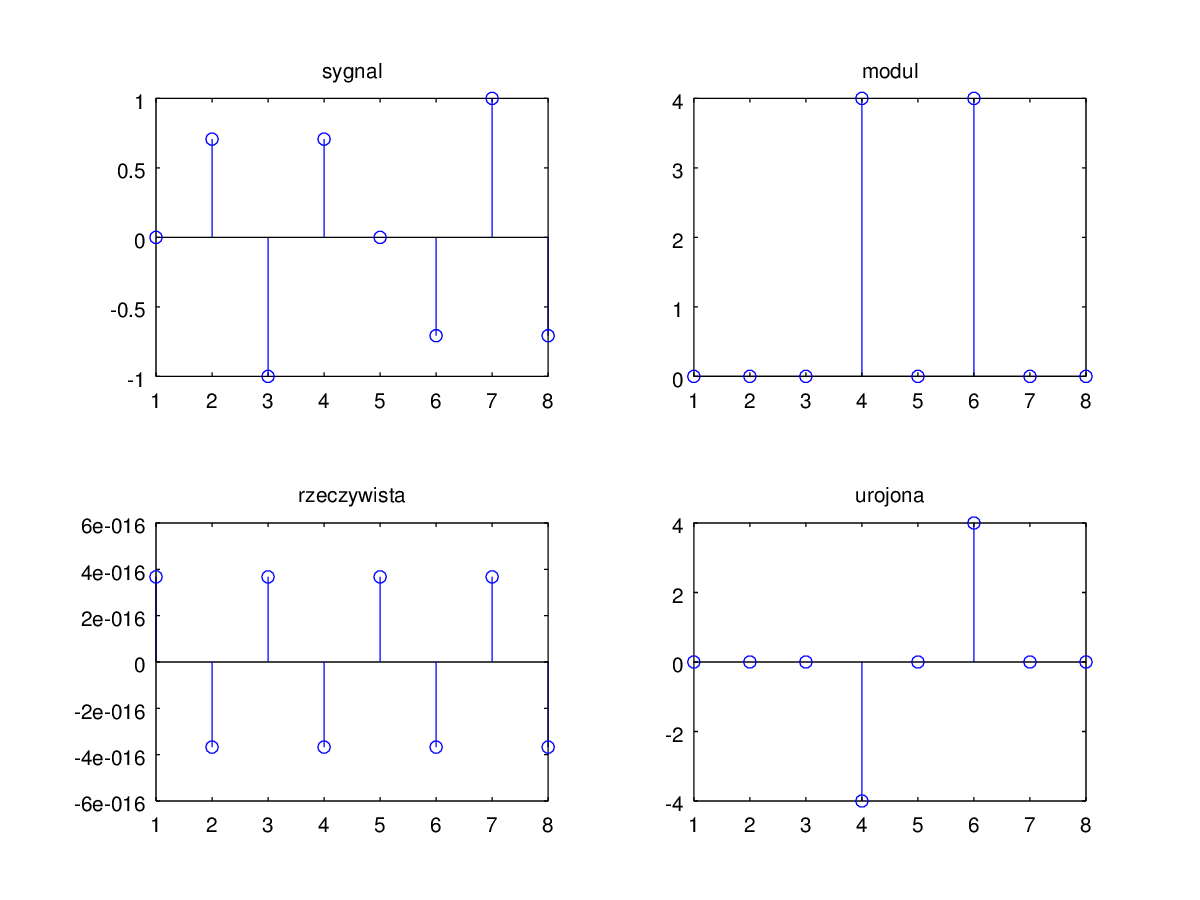
\includegraphics[scale=0.45]{../cw21_output_e}
	}
	\subfloat[]{
		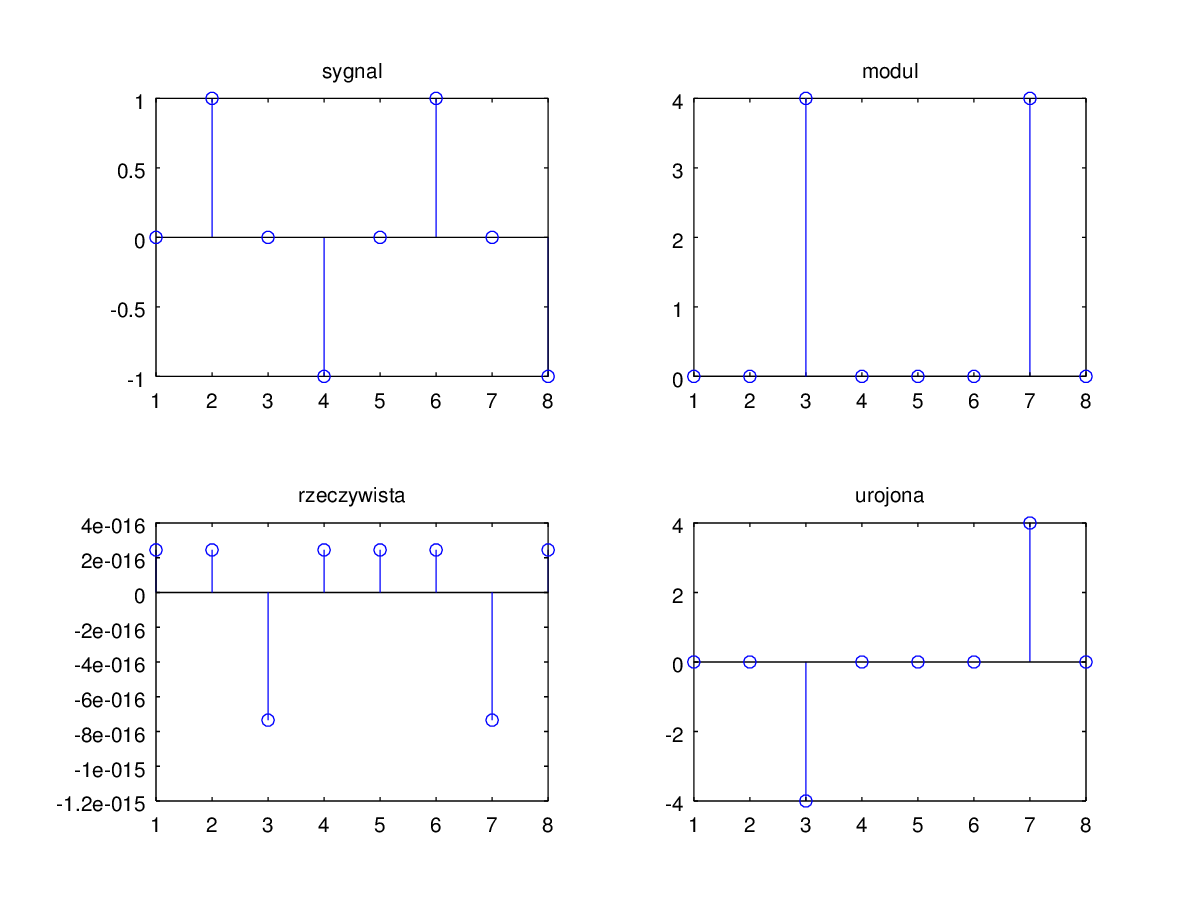
\includegraphics[scale=0.45]{../cw21_output_f}
	}
	\par
	\subfloat[]{
		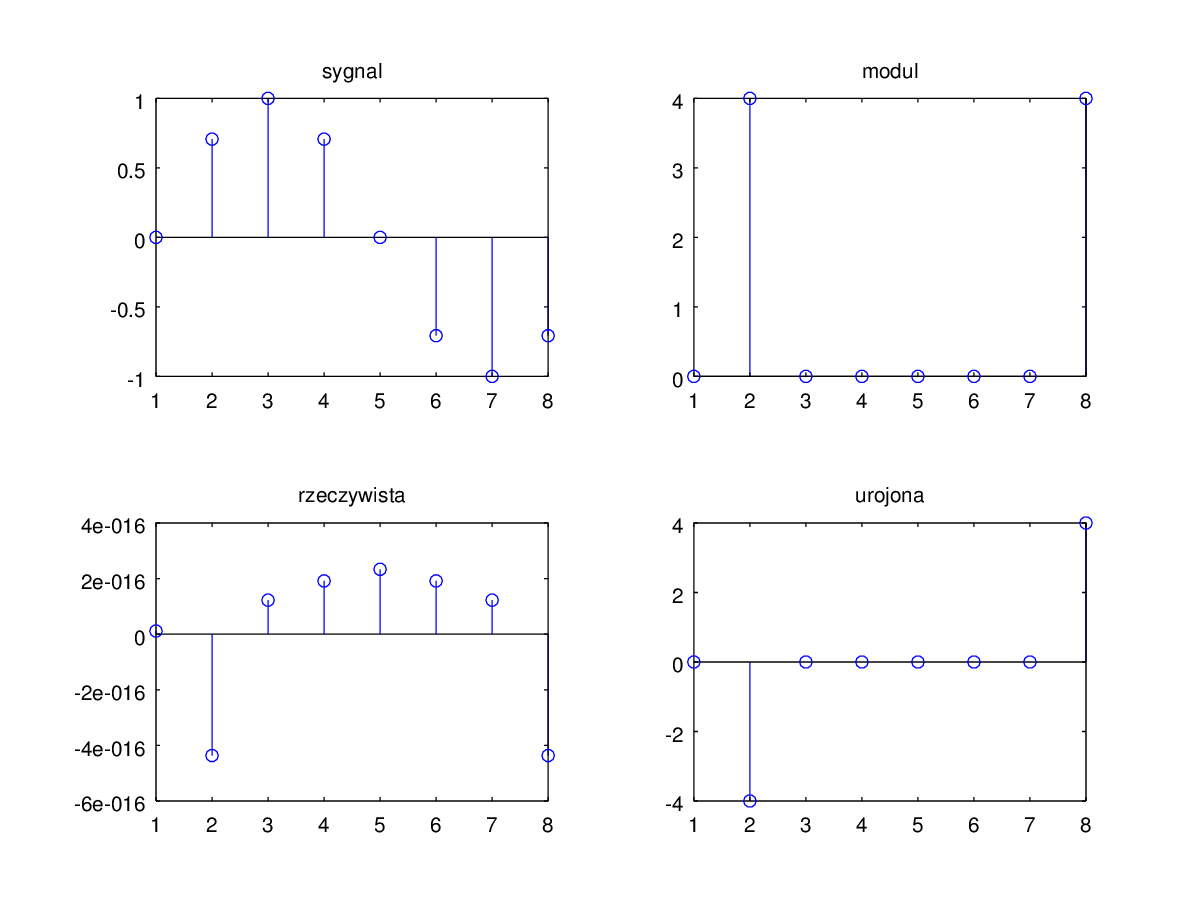
\includegraphics[scale=0.45]{../cw21_output_g}
	}
	\subfloat[]{
		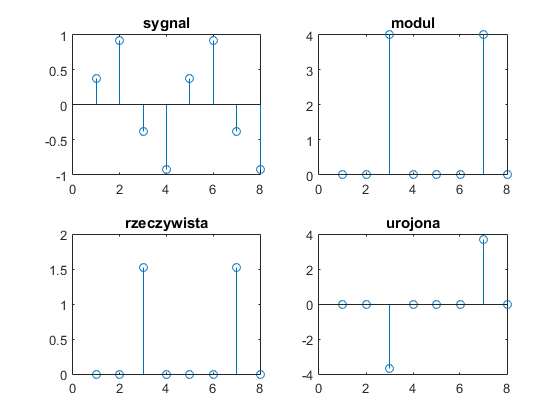
\includegraphics[scale=0.45]{../cw21_output_h}
	}
	\caption{Wyniki transformacji fourriera a - h}
\end{figure}
\begin{figure}
	\centering
	\subfloat[]{
		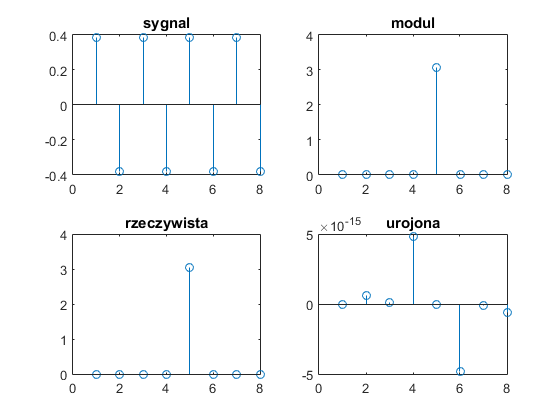
\includegraphics[scale=0.45]{../cw21_output_i}
	}
	\subfloat[]{
		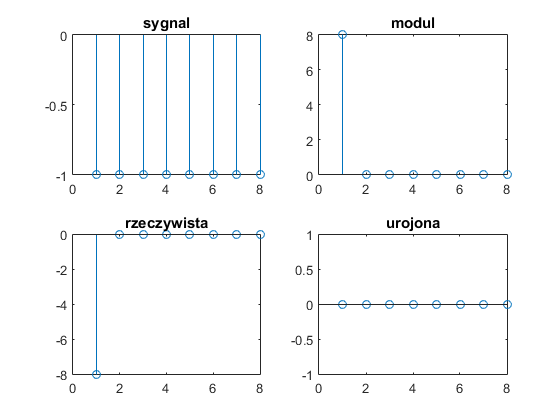
\includegraphics[scale=0.45]{../cw21_output_j}
	}
	\par
	\subfloat[]{
		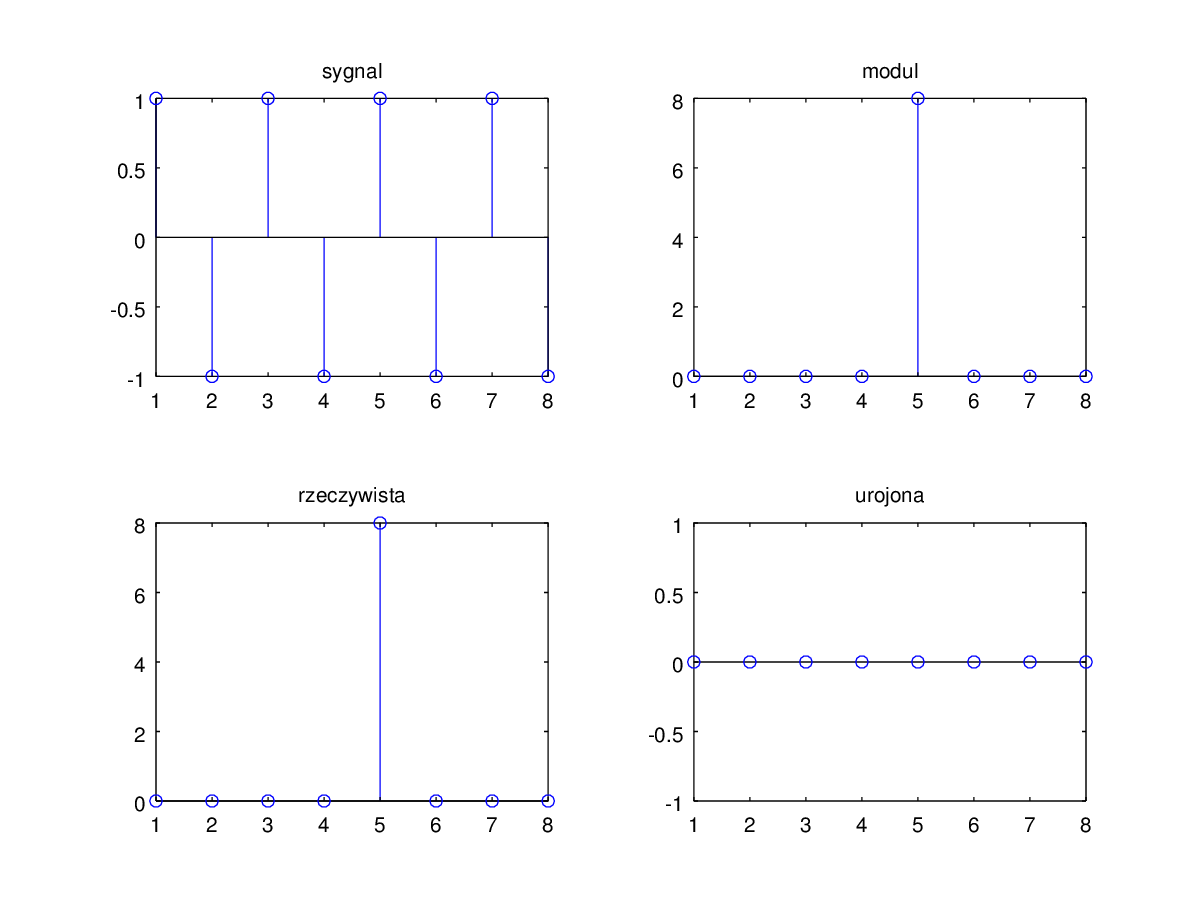
\includegraphics[scale=0.45]{../cw21_output_k}
	}
	\subfloat[]{
		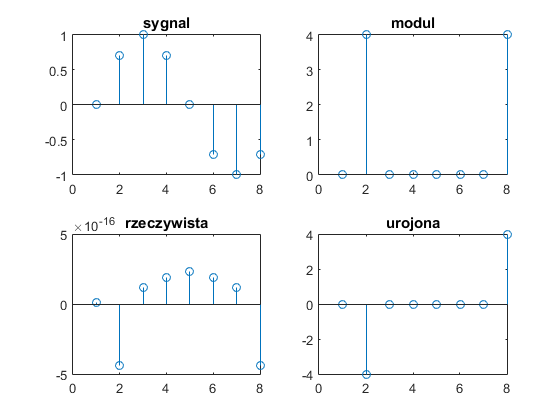
\includegraphics[scale=0.45]{../cw21_output_l}
	}
	\par
	\subfloat[]{
		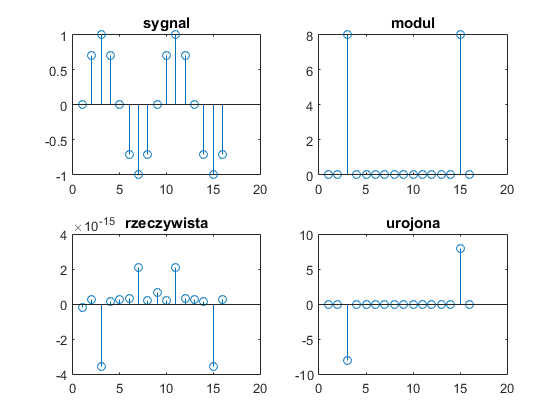
\includegraphics[scale=0.45]{../cw21_output_m}
	}
	\subfloat[]{
		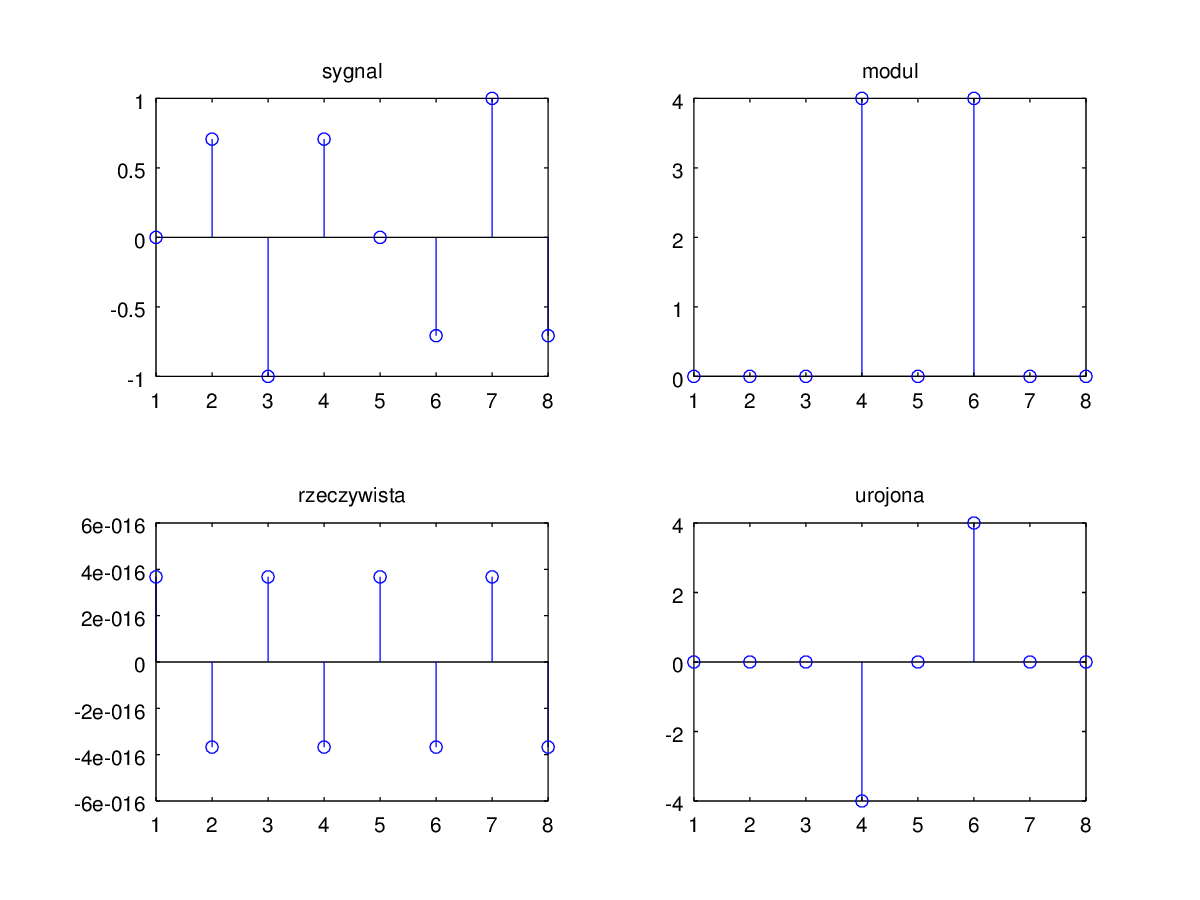
\includegraphics[scale=0.45]{../cw21_output_n}
	}
	\par
	\subfloat[]{
		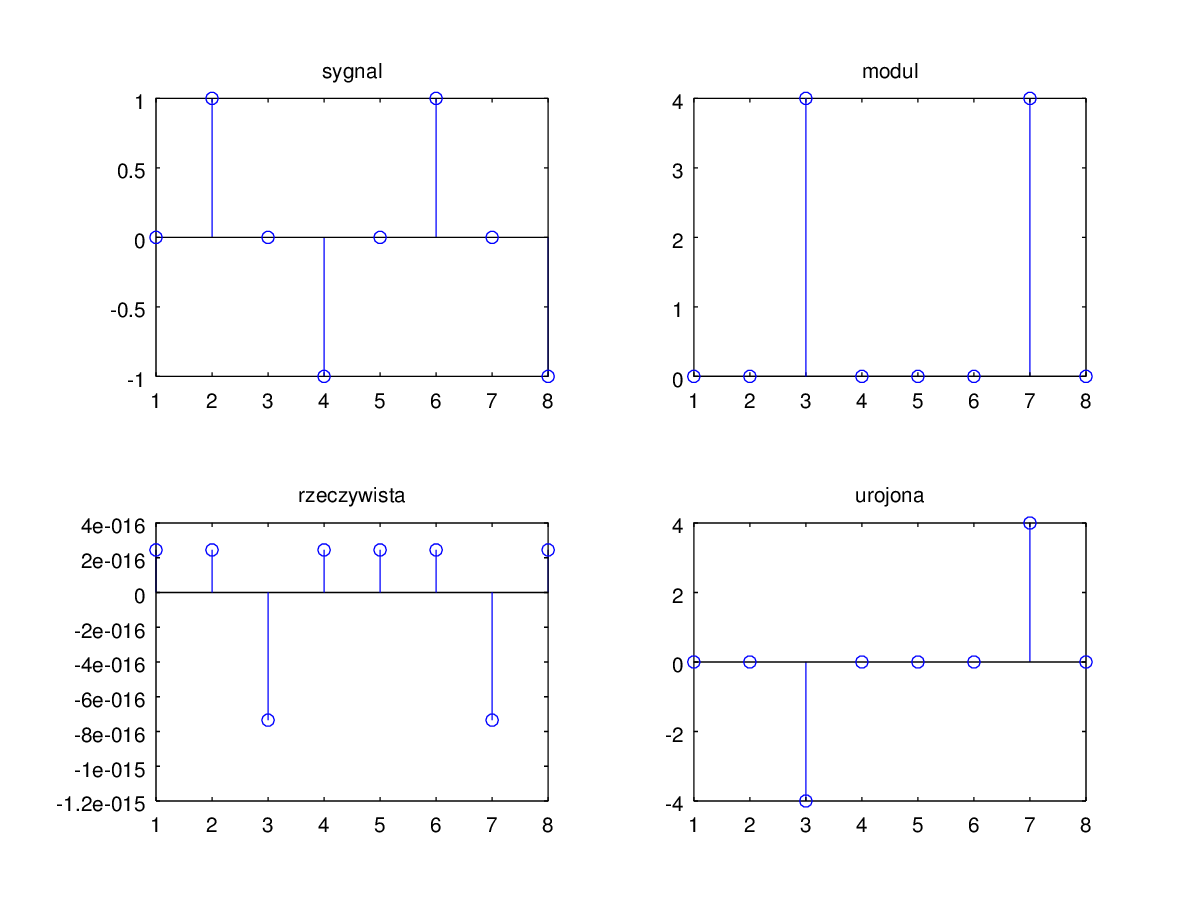
\includegraphics[scale=0.45]{../cw21_output_o}
	}
	\subfloat[]{
		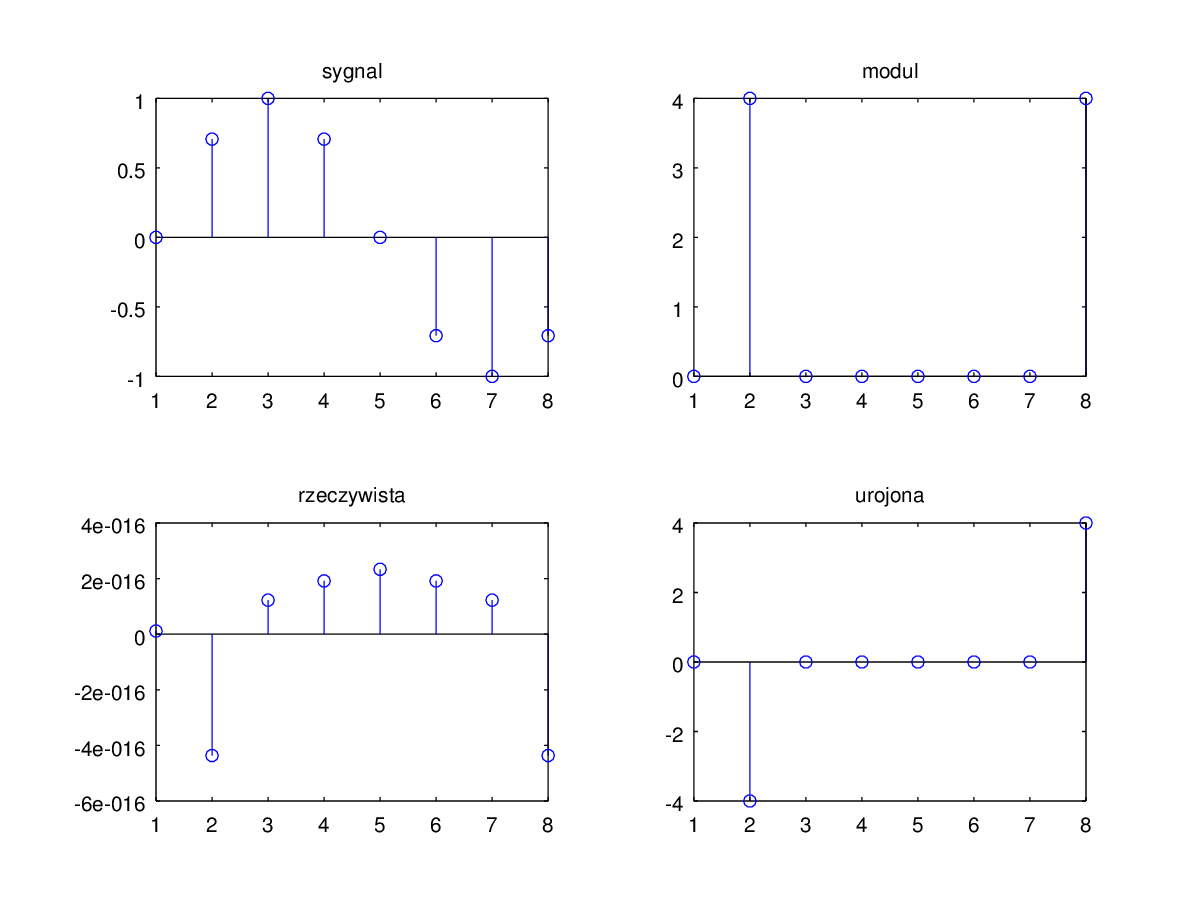
\includegraphics[scale=0.45]{../cw21_output_p}
	}
	\caption{Wyniki transfpormacji Fourriera i - p}
\end{figure}
\begin{figure}
	\centering
	\subfloat[]{
		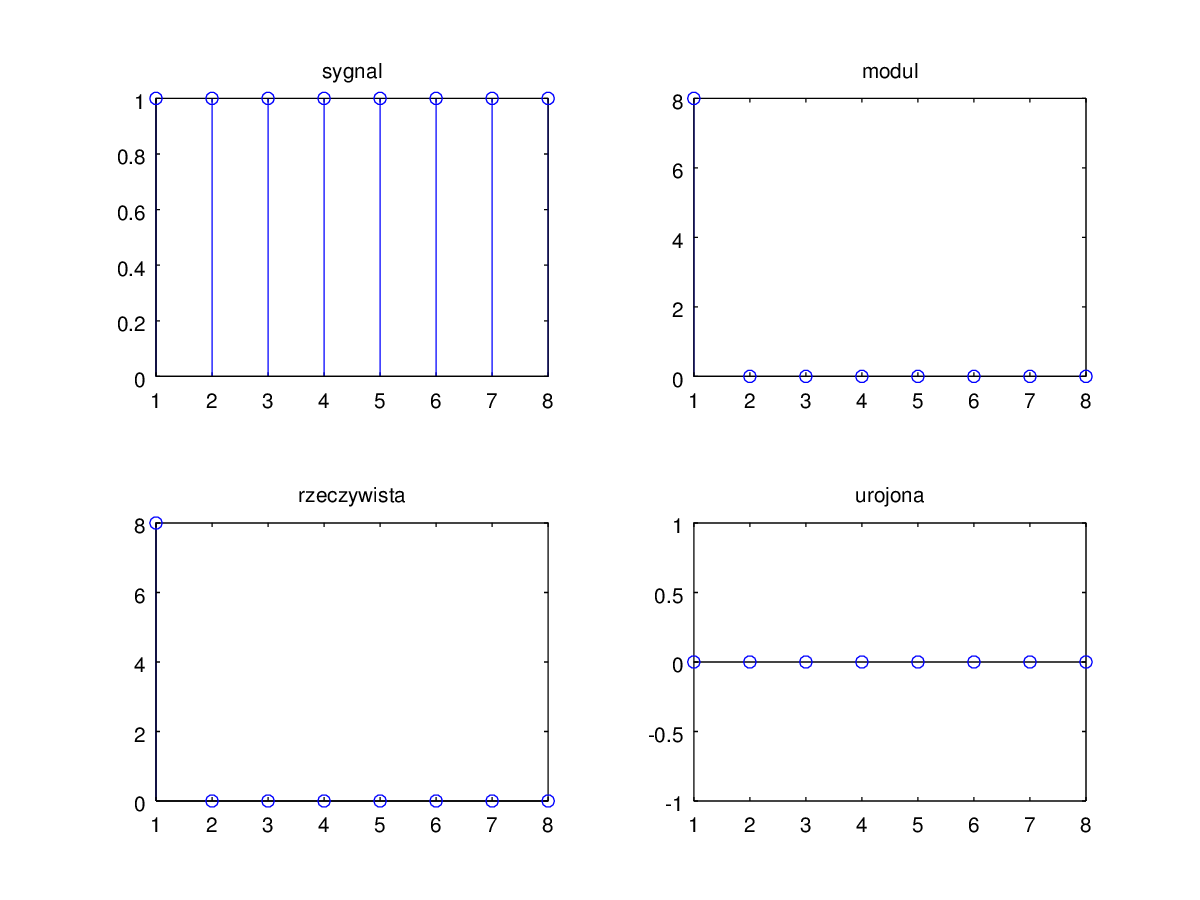
\includegraphics[scale=0.45]{../cw21_output_q}
	}
	\subfloat[]{
		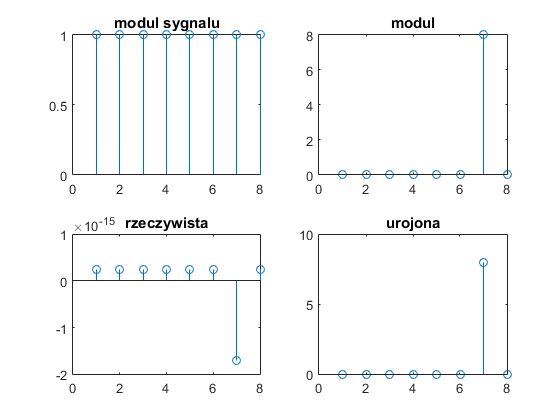
\includegraphics[scale=0.45]{../cw21_output_r}
	}
	\caption{Wyniki transformaty Fourriera q - r}
\end{figure}

Równania sygnałów:\\
\nolinebreak[4]
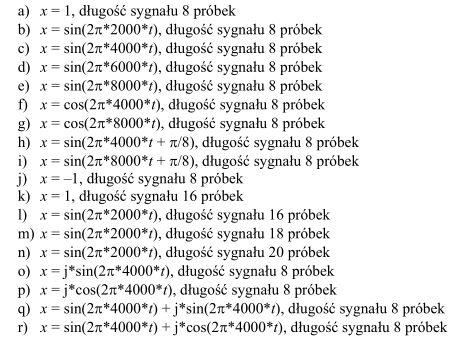
\includegraphics[scale=0.9]{../cw31_polecenie}\\
Różnica fazy nie wpływa na moduł transformaty Fourriera sygnału, zmienia natomiast jej część rzeczywistą co widać wyraźnie w przypadku sygnałów f i h z rysunku 11.Częstotliwość sygnału wyraźnie wpływa na położenie wysokiego prążka w module tranformaty.Transformata sygnalu urojonego (Rysunek 12, g) daje zamienione wartości dla składników rzeczywistego i urojonego w prównaniu dla transformaty analogicznego sygnału rzeczywistego (Rysunek 11, c).

\newpage
\subsection{Odwrotna DFT}
{
\scriptsize
\begin{verbatim}
figure
subplot(211);
stem(ones(1,8));
title("transformata");
subplot(212);
stem(abs(ifft(ones(1,8))));
title("transformata odwrotna");
\end{verbatim}
}
\begin{figure}[!h]
	\centering
	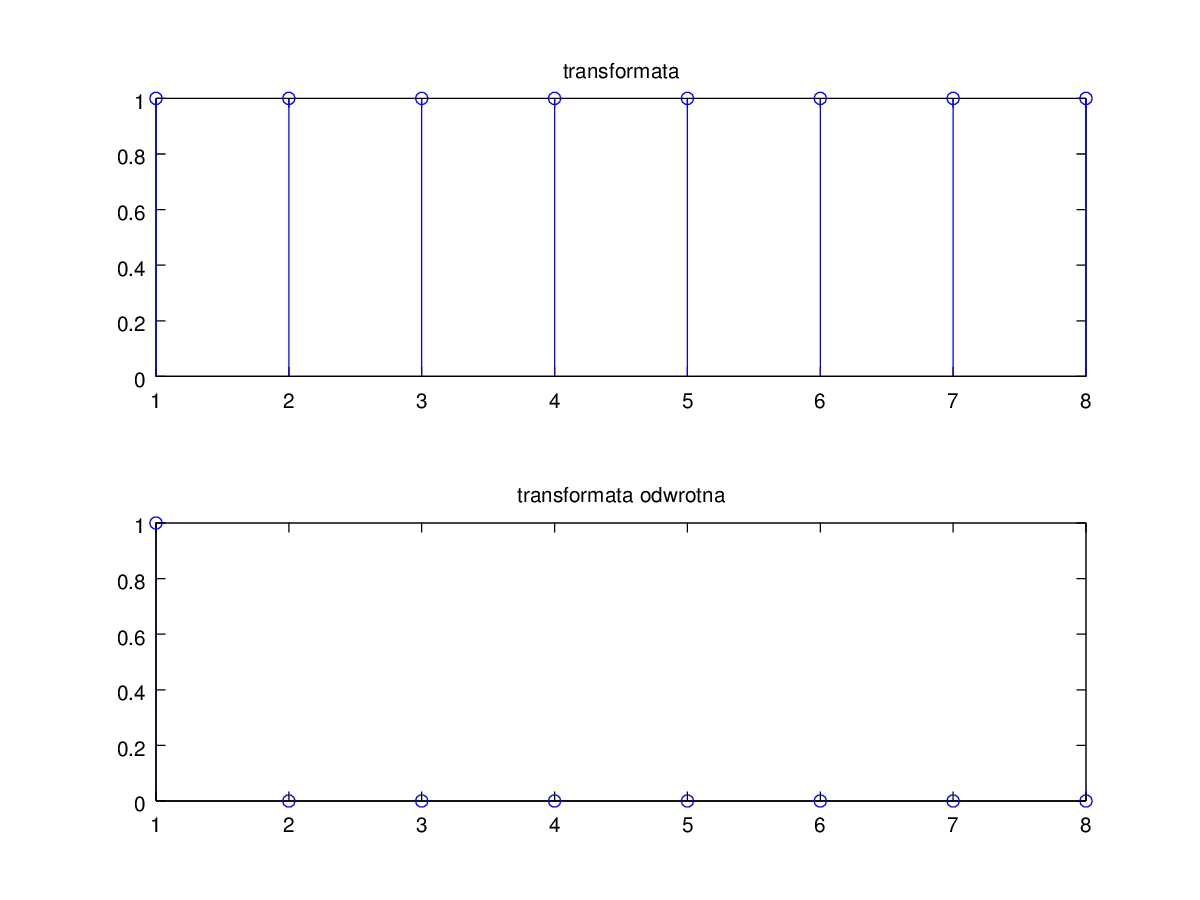
\includegraphics[scale=0.6]{../cw22_output}
	\caption{}
\end{figure}
Aby uzyskać sygnał dla którego wszystkie prążki widma będą równe jeden, wystarczy obliczyć transformatę odwrotną takiego wektora.
\newpage

\subsection{Rekonstrukcja sygnału z jego transformaty}
kod użyty do rekonstrukcji:
\begin{multicols}{3}
	{
		\footnotesize
		\begin{verbatim}
		a = [0,0,0,0,0,8,0,j*8,0,
			-j*8,0,8,0,0,0,0];
		x = ifft(a);
		x2 = [x,x,x,x,x,x,x,x];
		a2 = fft(x2);
		figure
		subplot(221);
		stem(real(a));
		hold on
		stem(imag(a), 'r');
		title("transformata sygnalu");
		subplot(222);
		stem(x);
		title("sygnal");
		subplot(223);
		stem(x2);
		title("wydluzony sygnal");
		subplot(224);
		stem(real(a2));
		hold on
		stem(imag(a2), 'r');
		title("transformata wydluzonego");
		\end{verbatim}
	}
\end{multicols}

\begin{figure}[!h]
	\centering
	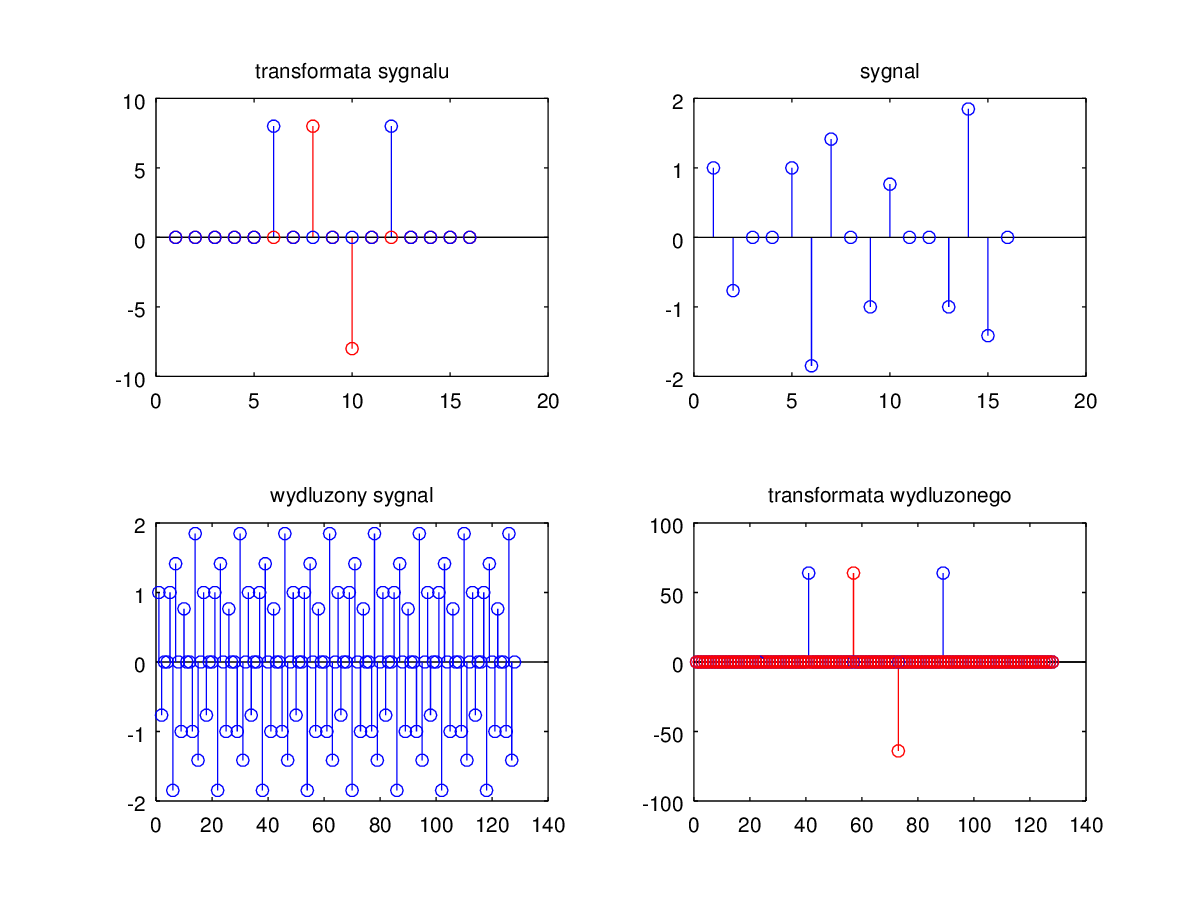
\includegraphics[scale=0.7]{../cw23_output}
	\caption{}
\end{figure}
Po wprowadzeniu transformaty synału wystarczy obliczyć jej odwrotną transformatę. Po parokrotnym skopiowaniu sygnału wynikowego i obliczeniu kontrolnej transformaty dochodzimy do wniosku, że metoda ta działa.
\newpage

\subsection{Okna Hamminga, Bartletta i Blackmana}
\begin{figure}[!h]
	\centering
	\subfloat[]{
		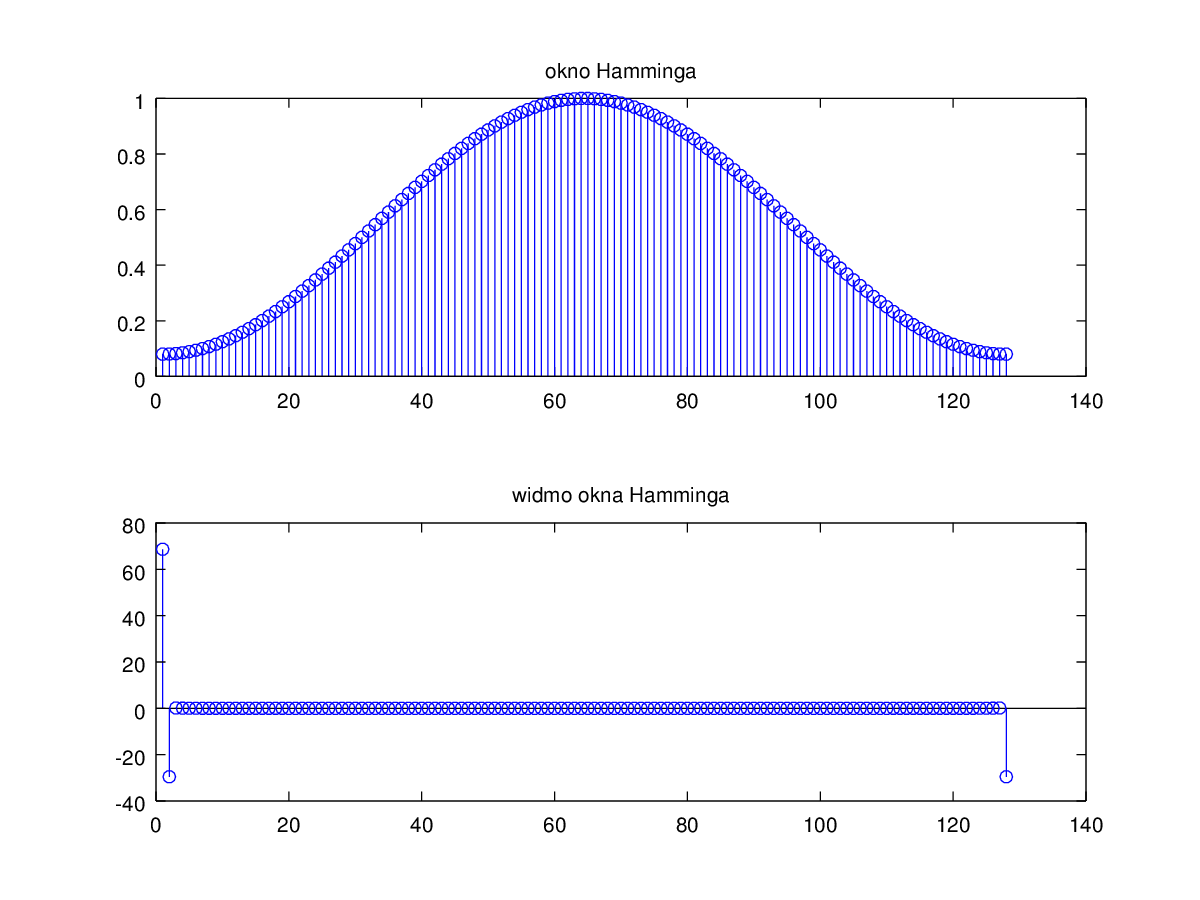
\includegraphics[scale=0.4]{../cw24_output_Hamming}
	}
	\subfloat[]{
		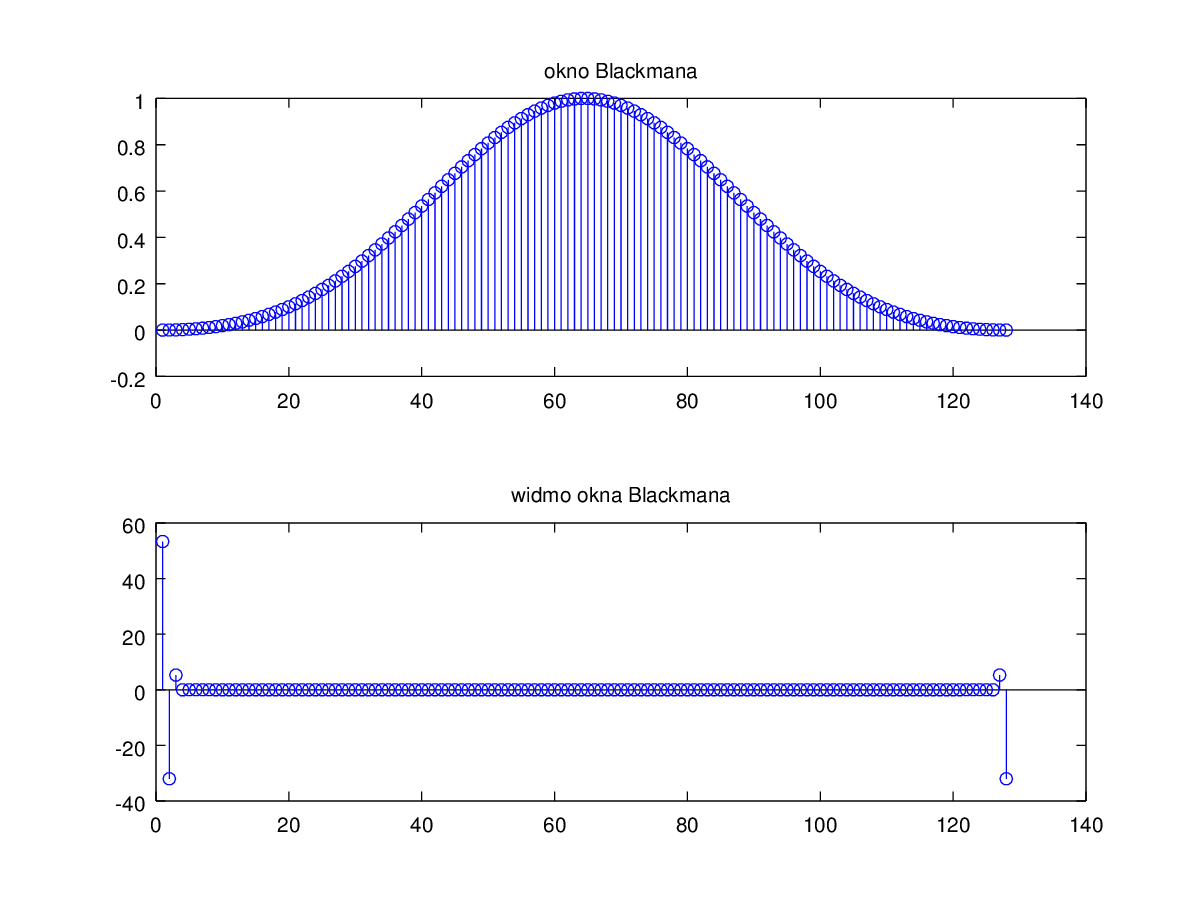
\includegraphics[scale=0.4]{../cw24_output_blackman}
	}
	\par
	\subfloat[]{
		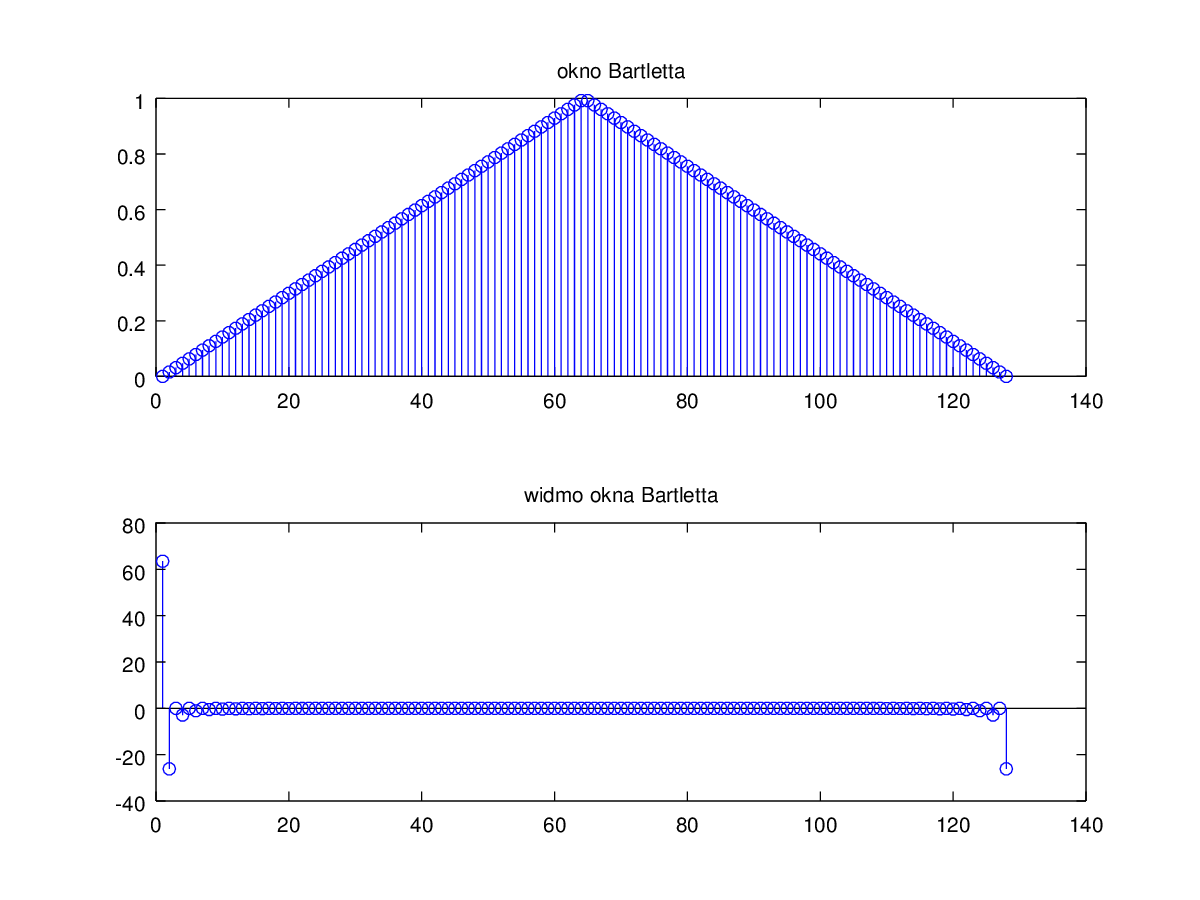
\includegraphics[scale=0.4]{../cw24_output_Bartlett}
	}
	\caption{Kształty okien i ich widma}
\end{figure}
Okno Bartletta jest na pierwszy rzut oka najprostsze i wydaje się być najmniej przydatne z powyższych okien. Najbardziej równomierne widmo ma natomiast okno Hamminga i wydaje się być najbardziej użyteczne.
\newpage

\subsection{Uzycie okien do obserwacji widm przebiegów}
Obserwowane sygnały:
\begin{figure}[!h]
	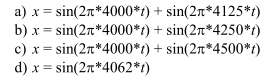
\includegraphics[scale=0.7]{../cw25_polecenie}
\end{figure}
Skrypt użyty do generacji przebiegów:
\begin{multicols}{3}
	{
		\tiny
		\begin{verbatim}
		%sampling frequency
		fs=16000;
		
		%samples vector
		n=[0:127];
		
		%time vectors
		t=n/fs;
		
		%signal model
		xa=sin(2*pi*4000*t)+sin(2*pi*4125*t);
		xb=sin(2*pi*4000*t)+sin(2*pi*4250*t);
		xc=sin(2*pi*4000*t)+sin(2*pi*4500*t);
		xd=sin(2*pi*4062*t);
		
		%windows
		ham = rot90(hamming(128));
		bla = rot90(blackman(128));
		bar = rot90(bartlett(128));
		
		figure
		subplot(231);
		stem(xd);
		title("sygnal wejsciowy");
		subplot(234);
		stem(xd.*ham);
		title("sygnal wejsciowy po oknie Hamminga");
		subplot(2,3,[2,3]);
		stem(abs(fft(xd)));
		title("widmo sygnalu");
		subplot(2,3,[5,6]);
		stem(abs(fft(xd.*ham)));
		title("widmo sygnalu po oknie Hamminga");
		
		figure
		subplot(231);
		stem(xd);
		title("sygnal wejsciowy");
		subplot(234);
		stem(xd.*bla);
		title("sygnal wejsciowy po oknie Blackmana");
		subplot(2,3,[2,3]);
		stem(abs(fft(xd)));
		title("widmo sygnalu");
		subplot(2,3,[5,6]);
		stem(abs(fft(xd.*bla)));
		title("widmo sygnalu po oknie Blackmana");
		
		figure
		subplot(231);
		stem(xd);
		title("sygnal wejsciowy");
		subplot(234);
		stem(xd.*bar);
		title("sygnal wejsciowy po oknie Bartletta");
		subplot(2,3,[2,3]);
		stem(abs(fft(xd)));
		title("widmo sygnalu");
		subplot(2,3,[5,6]);
		stem(abs(fft(xd.*bar)));
		title("widmo sygnalu po oknie Bartletta");
		\end{verbatim}
	}
\end{multicols}

\begin{figure}[!h]
	\centering
	\subfloat[]{
		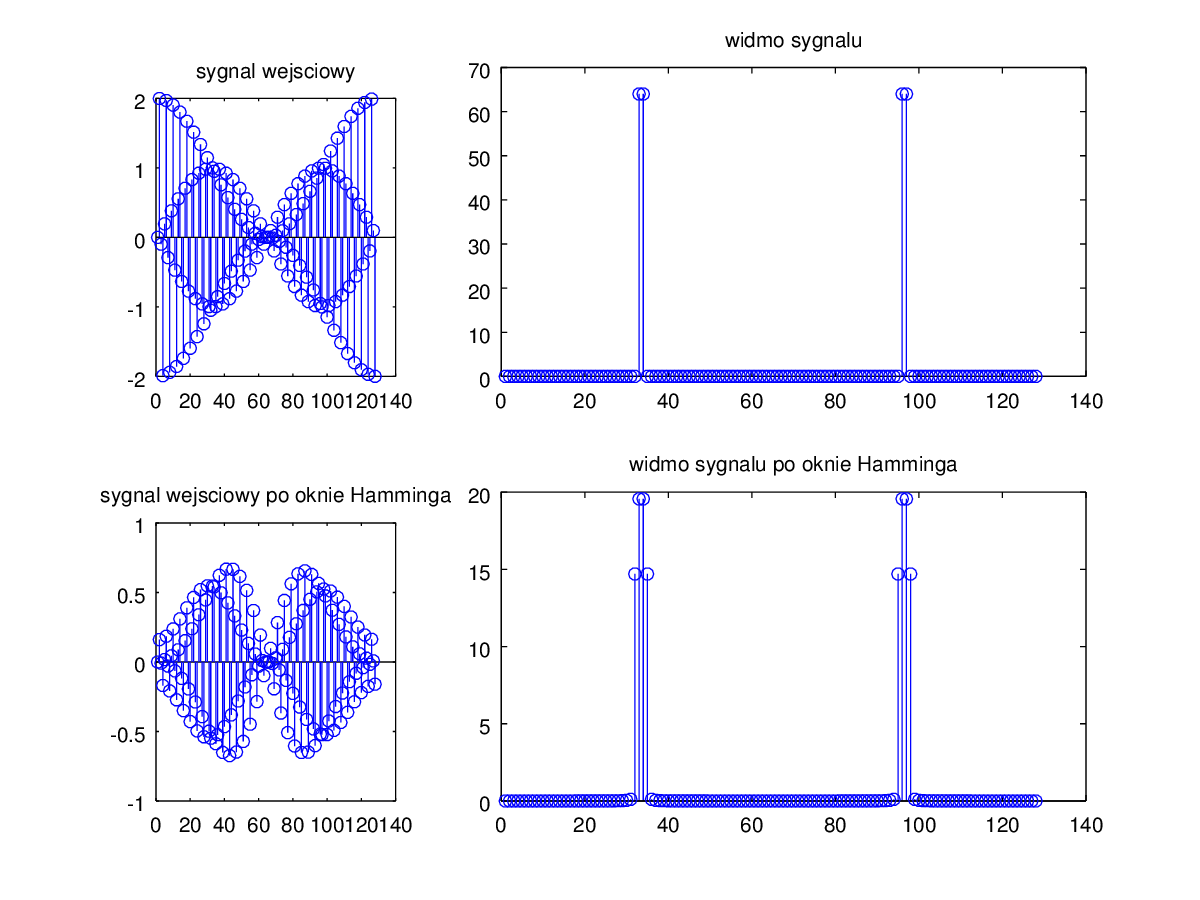
\includegraphics[scale=0.4]{../cw25_output_A_Hamming}
	}
	\subfloat[]{
		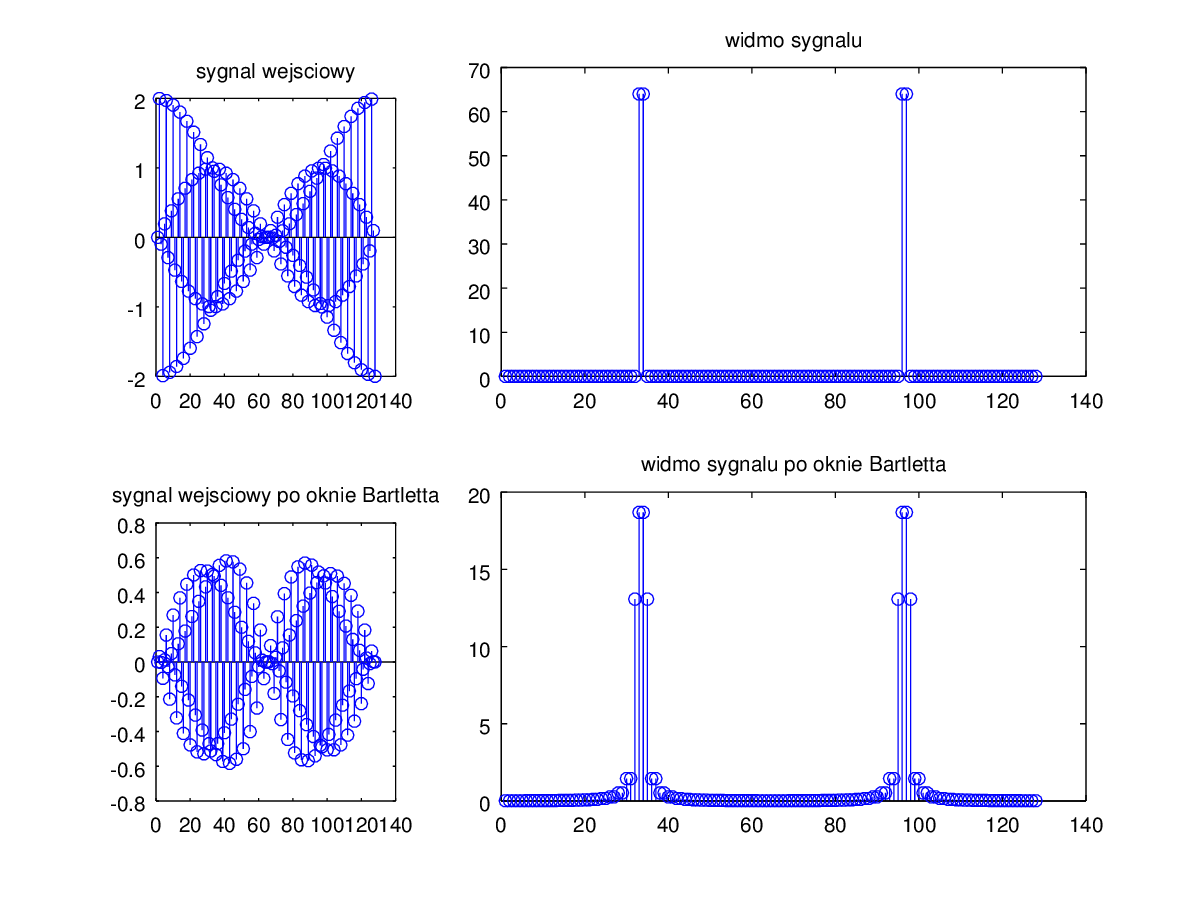
\includegraphics[scale=0.4]{../cw25_output_A_Bartlett}
	}
	\caption{Obserwacja sygnału A przez okna Hamminga i Bartletta}
\end{figure}

Widoczna jest większa przydatność okna Hamminga, gdyż okno Bartletta wprowadza zbyt duże zniekształcenia.

\begin{figure}[!h]
	\centering
	\subfloat[]{
		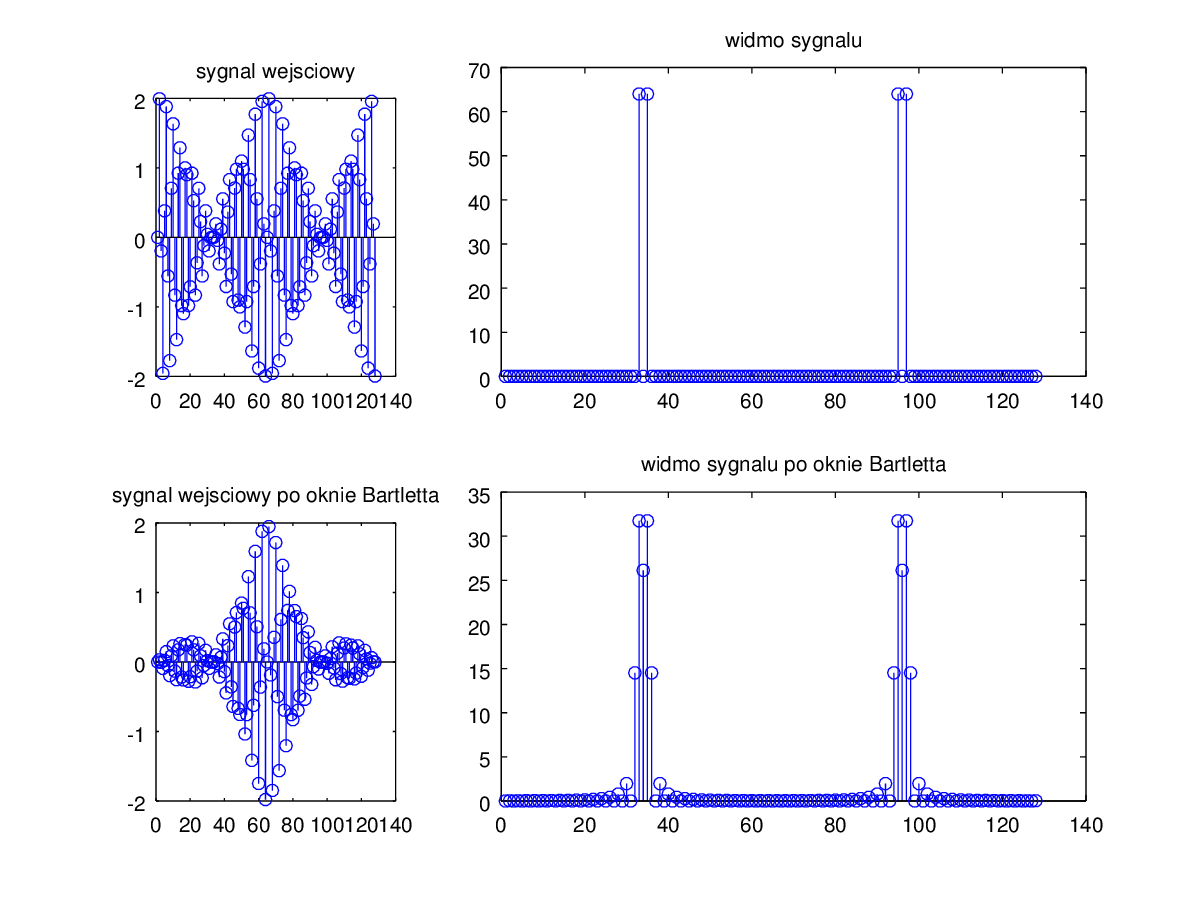
\includegraphics[scale=0.3]{../cw25_output_B_Bartlett}
	}
	\subfloat[]{
		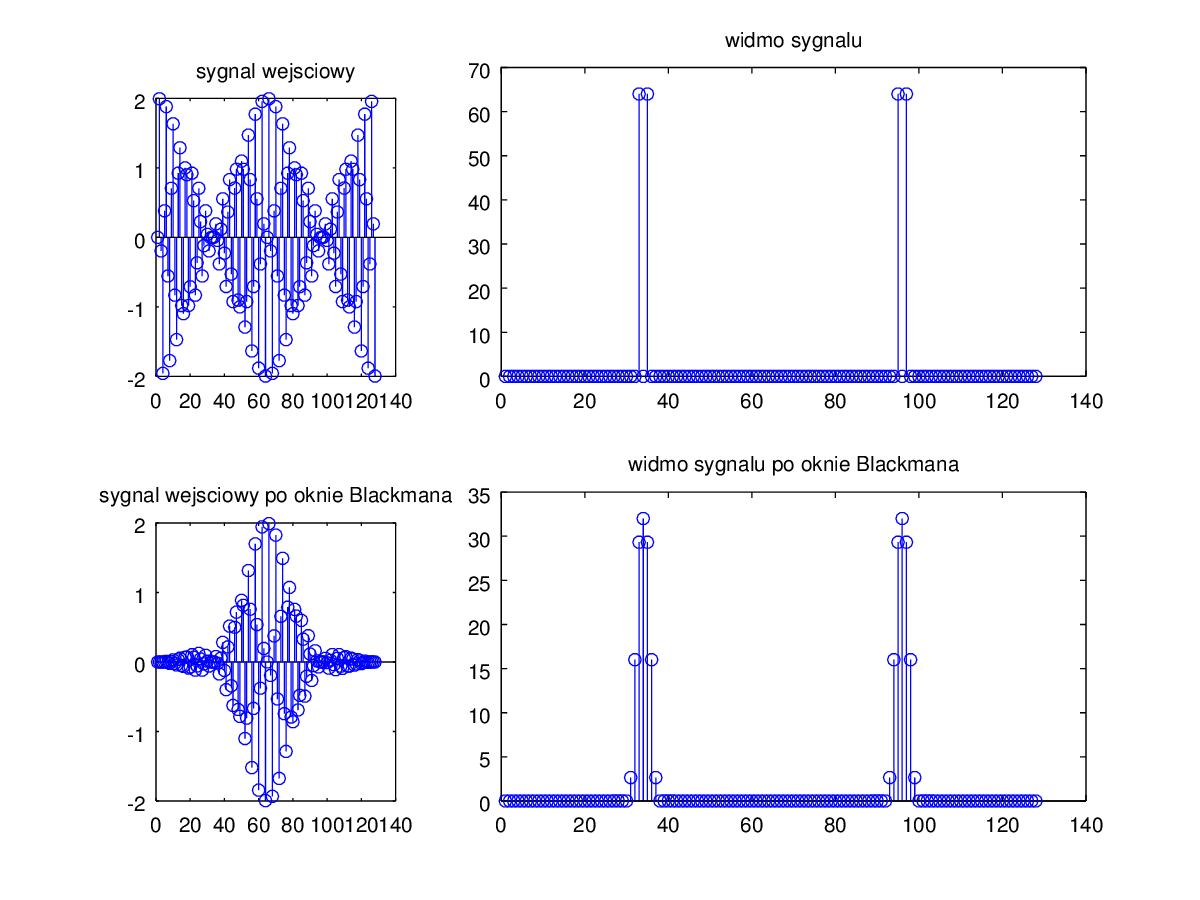
\includegraphics[scale=0.3]{../cw25_output_B_Blackman}
	}
	\caption{Obserwacja sygnału B przez okna Bartletta i Blackmana}
\end{figure}

Zarówno okno Bartletta i Blackmana wprowadzają zauważalne zniekształcenia sygnału, lecz okno Blackmana jest odrobinę lepsze pod tym względem.
\newpage

\begin{figure}[!h]
	\centering
	\subfloat[]{
		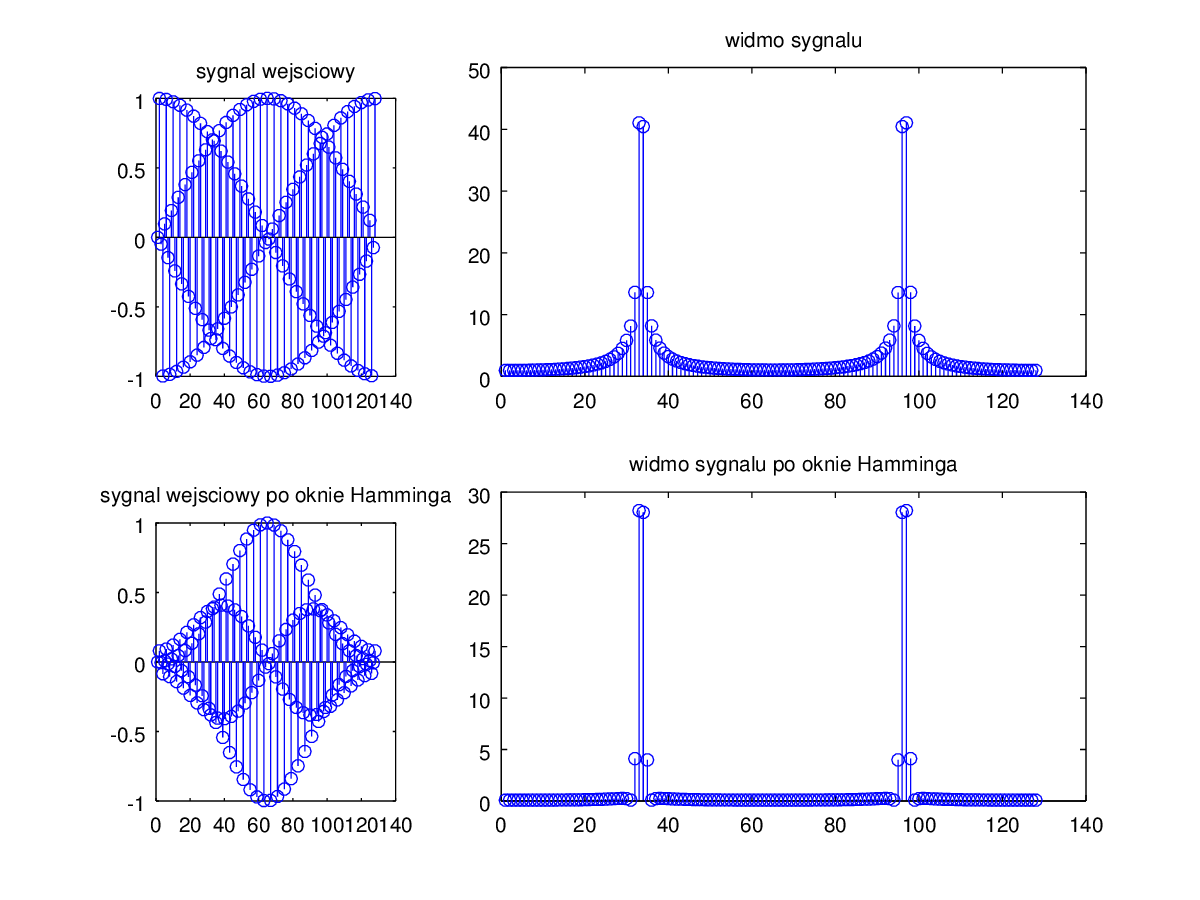
\includegraphics[scale=0.4]{../cw25_output_D_Hamming}
	}
	\subfloat[]{
		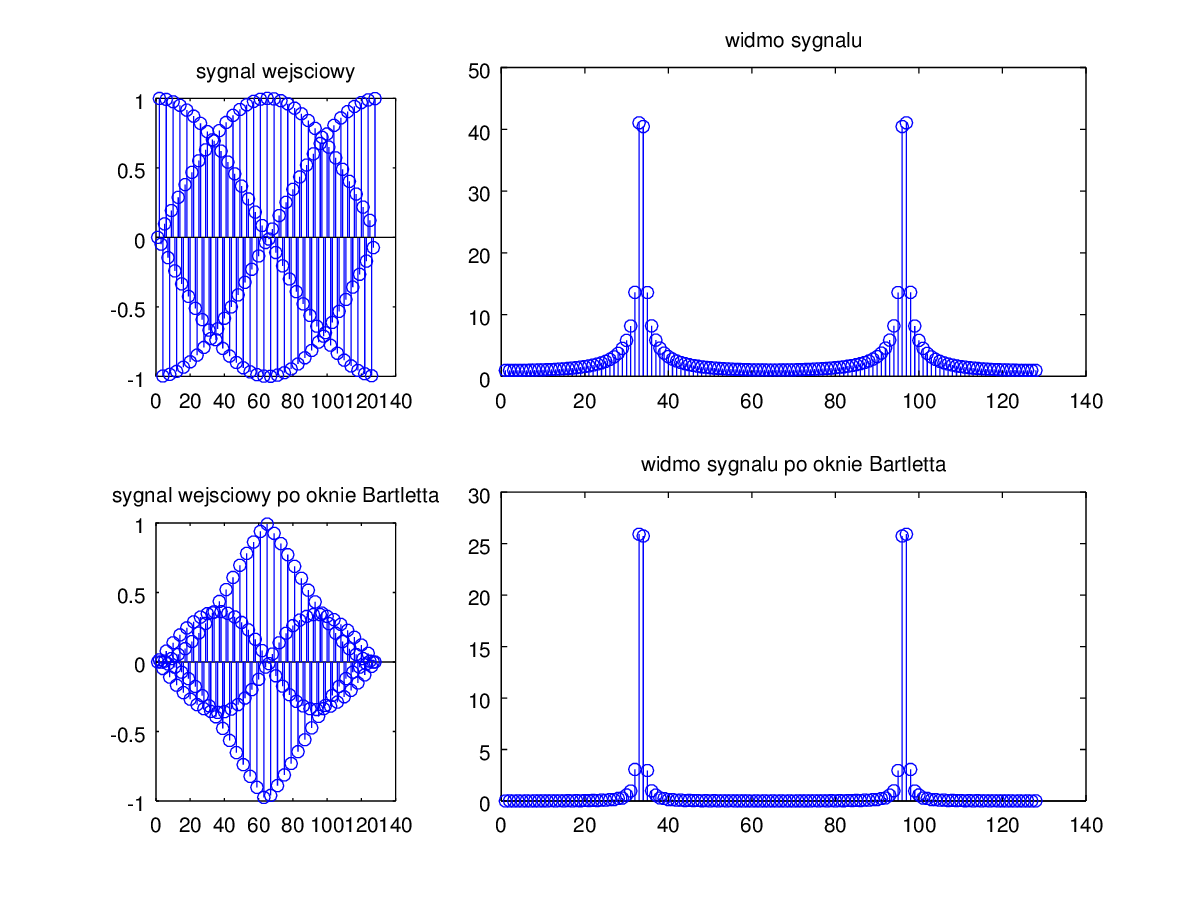
\includegraphics[scale=0.4]{../cw25_output_D_Bartlett}
	}
	\par
	\subfloat[]{
		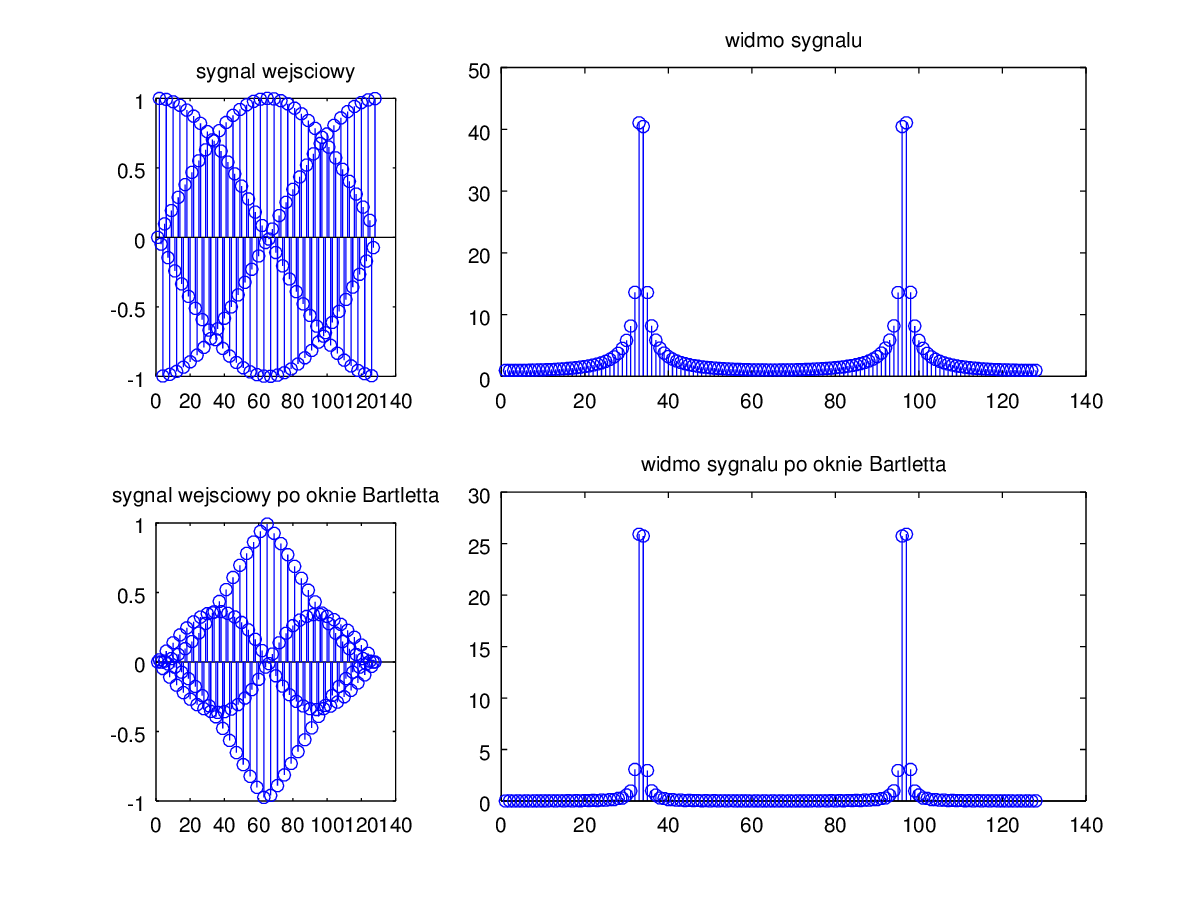
\includegraphics[scale=0.4]{../cw25_output_D_Bartlett}
	}
	\caption{Obserwacja sygnału D przez okna Hamminga, Bartletta i Blackmana}
\end{figure}
Dla poprzednich sygnałów nie występował przeciek widma ze względu na częstotliwości sygnałóW dopasowane do częstotliwości próbkowania. Okna skutkowały wtedy tylko wprowadzeniem zniekształceń. W przypadku sygnału D występuje duży przeciek i okna mogą mu zapobiec. Tak jak przewidywałem, okno Hamminga okazuje się być najbardziej przydatne
\par
Jak widać, okna moga wprowadzać niepożądane czestotliwości i czynić pomiar mniej dokładnym. W większości przypadków jednak okażą się bardzo pomocne.
\newpage

\section{Filtry SOI}
\subsection{Filtr dolnoprzepustowy}
Skrypt użyty do projektowania filtru i przefiltrowania sygnału kwadratowego:
\begin{multicols}{3}
	{
		\tiny
		\begin{verbatim}
		n = [-16:16]; %rzad filtru
		
		ft = 5500; %czestotliwosc graniczna
		fs = 16000;
		
		wg = 2*pi*ft/fs;
		h = (wg/pi)*sinc(wg*n/pi); %odpowiedz impulsowa
		w = blackman(33)';
		hw = h.*w;
		freqz(hw,1,512,fs);
		
		%samples vector
		na=[0:127];
		
		%signal frequency
		f=500;
		
		%time vectors
		t=na/fs;
		
		%signal model
		a=sin(2*pi*f*t);
		xa=sign(a);
		
		xf = filter2(hw, xa);
		
		figure
		subplot(211)
		plot(xa)
		subplot(212)
		plot(xf)
		\end{verbatim}
	}
\end{multicols}
\begin{figure}[!h]
	\centering
	\subfloat[Okno Hamminga]{
		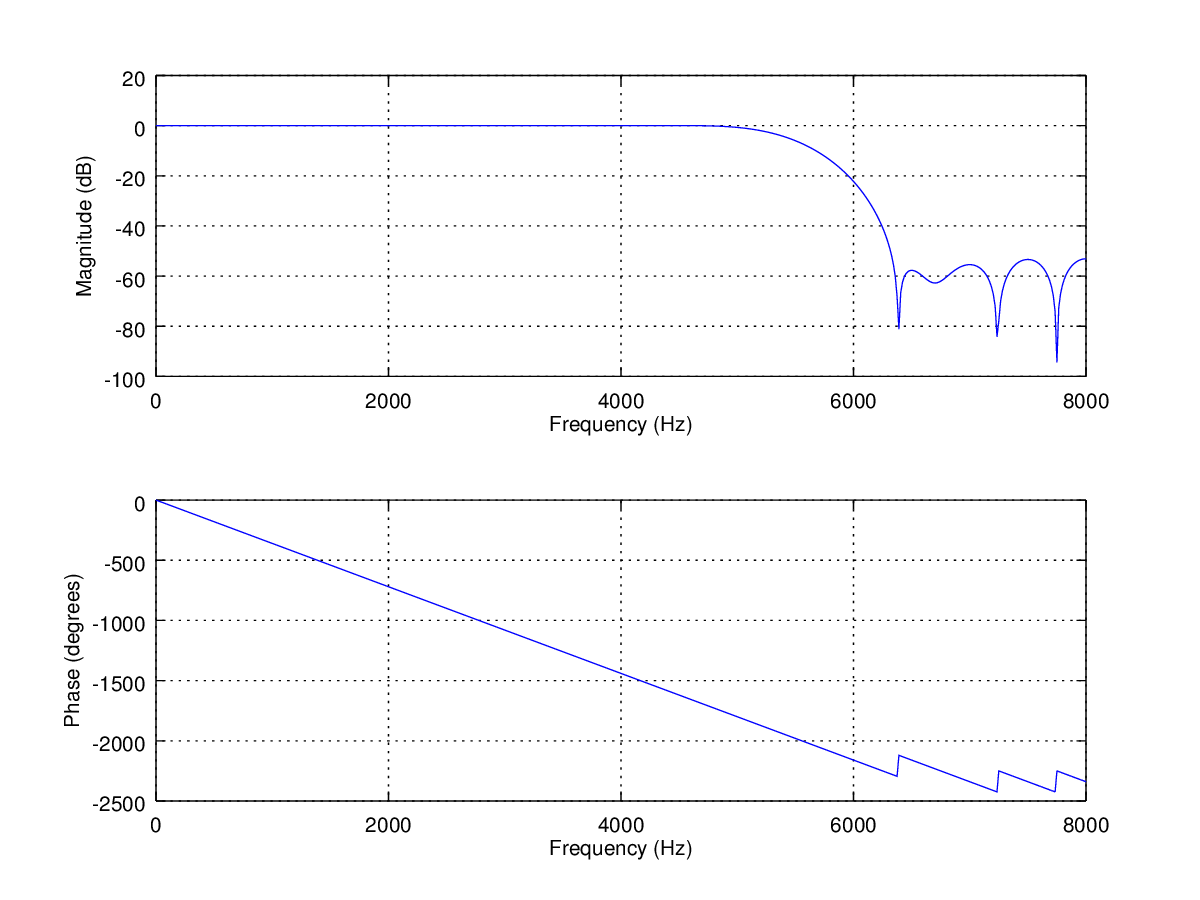
\includegraphics[scale=0.4]{../cw31_output_17_Hamming}
	}
	\subfloat[Okno Bartletta]{
		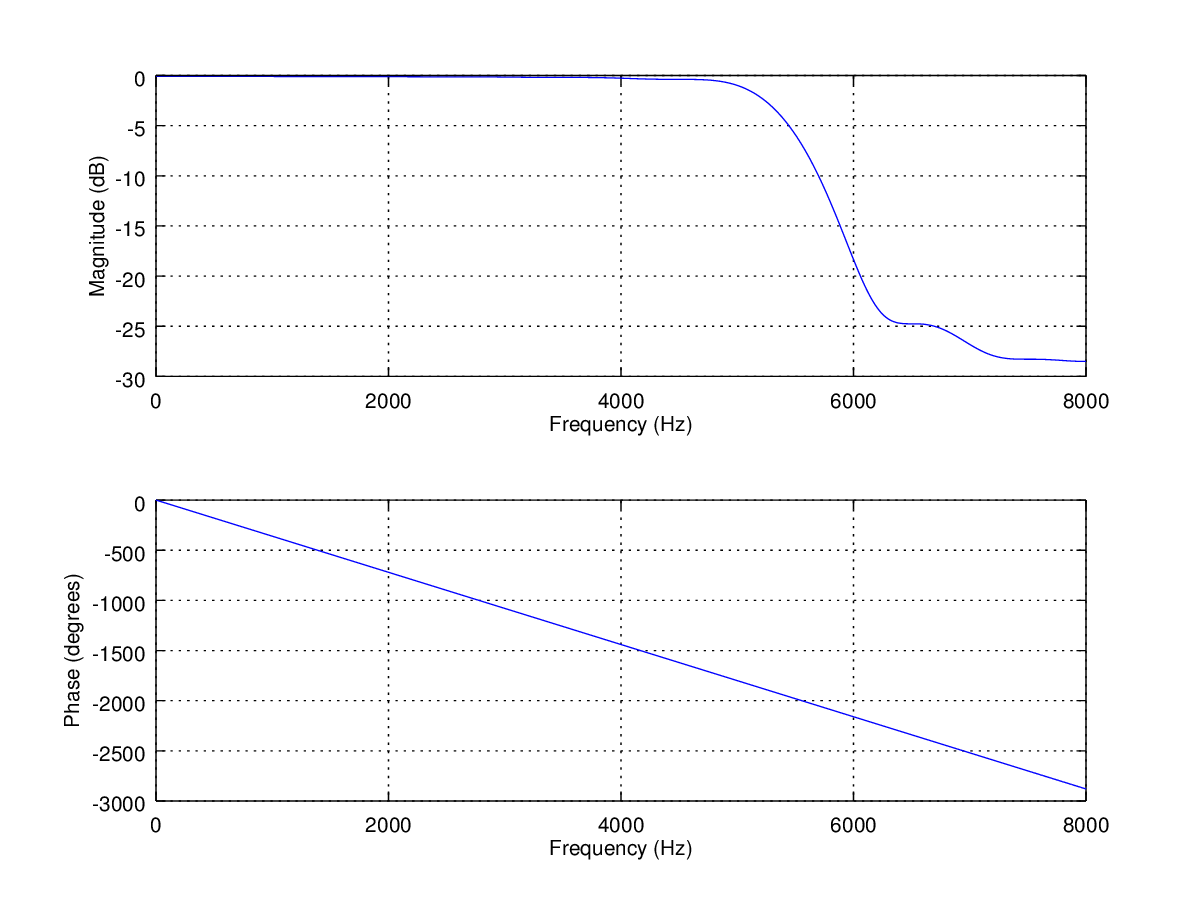
\includegraphics[scale=0.4]{../cw31_output_17_Bartlett}
	}
	\par
	\subfloat[okno Blackmana]{
		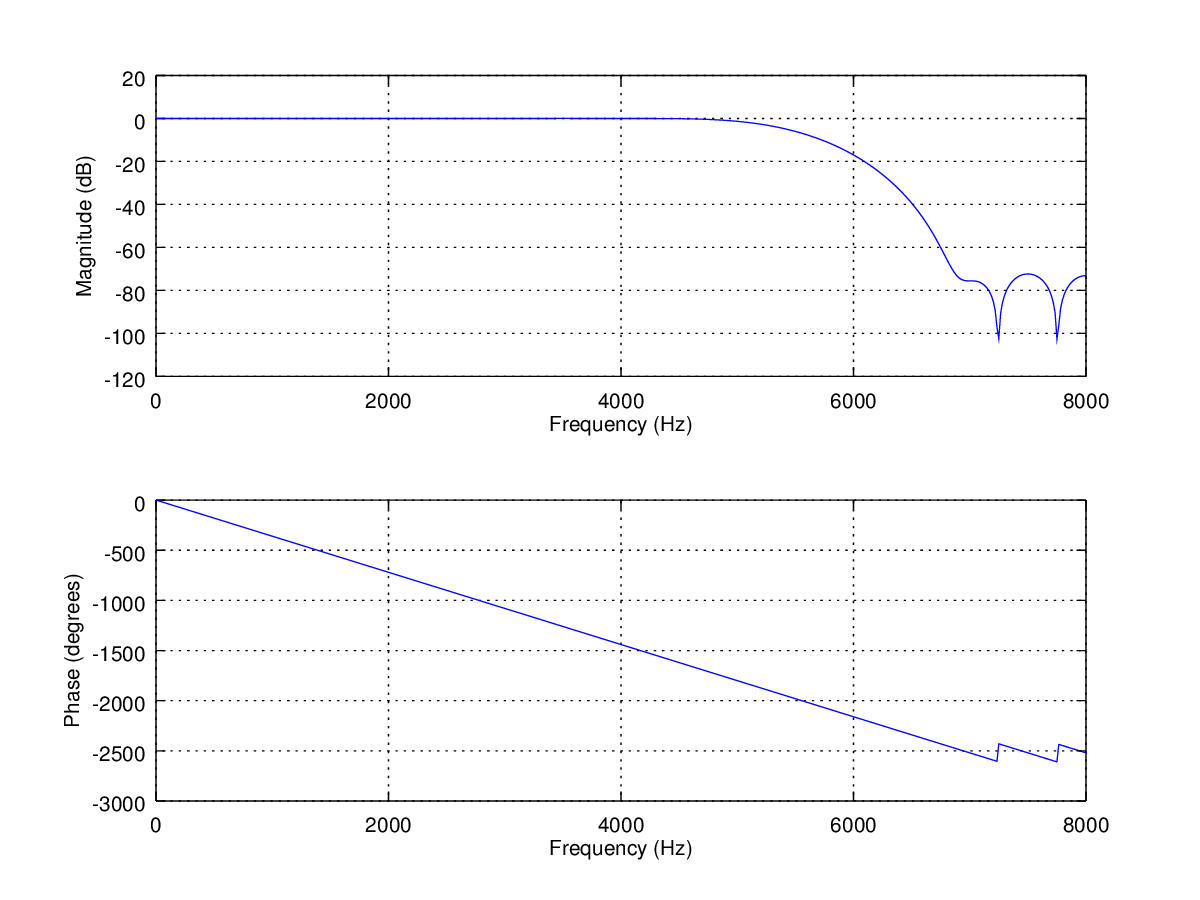
\includegraphics[scale=0.4]{../cw31_output_17_Blackman}
	}
	\caption{Charakterystyki projektowanych filtrów rzędu 17}
\end{figure}
W przypadku filtru 17 rzędu okno Blackmana zapewnia największe tłumienie w paśmie zaporowym poniżej -80 dB ze stosunkowo niewielką amplitudą listków bocznych w porównaniu do okna Hamminga. Okno Bartleta ma najmniejszą amplitudę listków bocznych, alecz również niewielkie tłumienie.
\newpage
\begin{figure}[!h]
	\centering
	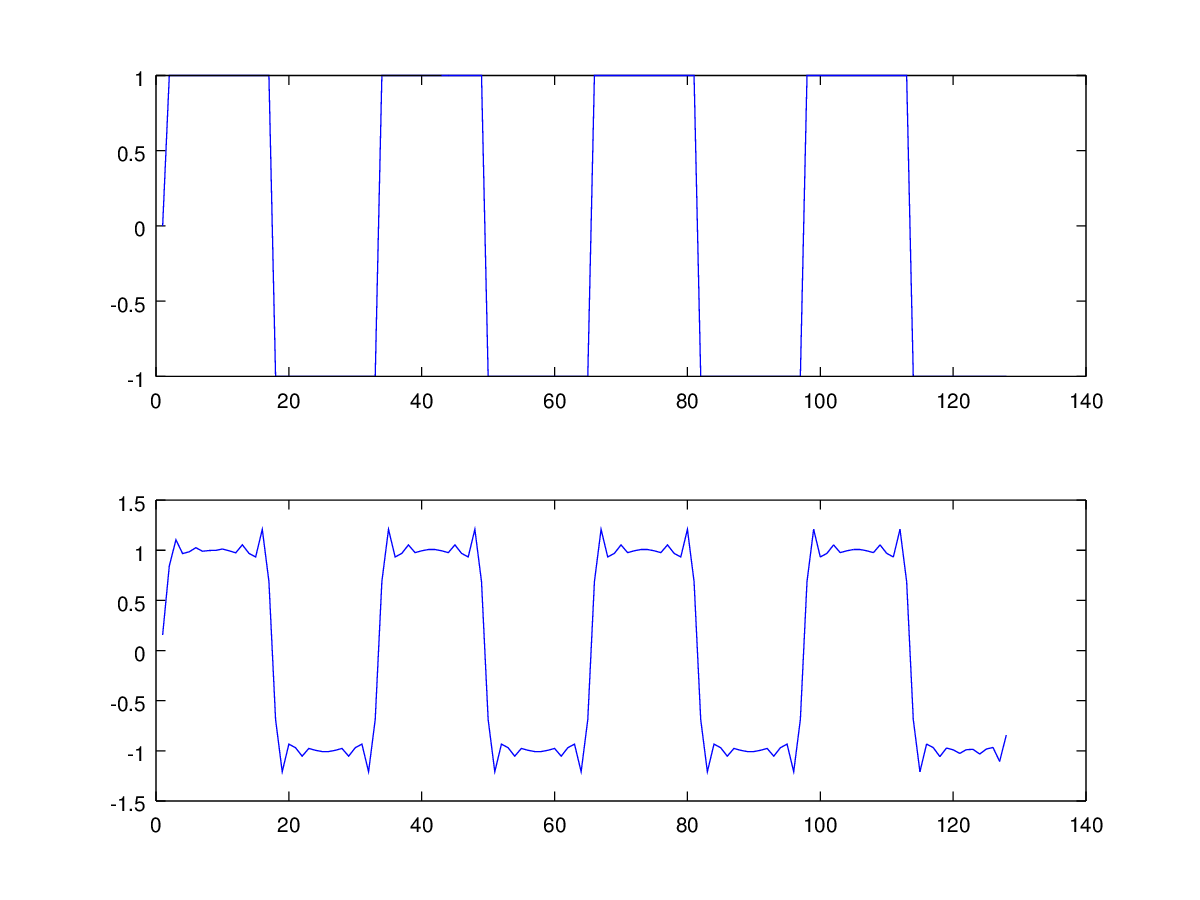
\includegraphics[scale=0.7]{../cw31_output_kwadrat_Blackman_plot}
	\caption{Przebieg kwadratowy i wynik filtrowania dolnoprzepustowego z oknem Blackmana}
\end{figure}
Wybrałem okno Blackmana ponieważ daje ono niską amplitudę listków bocznych. Aby uzyskać wymagane 70 dB tłumienia w paśmie zaporowym zwiększyłem rząd filtru z 17 do 33.
\newpage

\subsection{Filtr pasmowo-przepustowy}
Skrypt użyty do projektowania filtru:
\begin{multicols}{3}
	{
		\tiny
		\begin{verbatim}
		n = [-16:16]; %rzad filtru
		
		ft = 6000; %czestotliwosc graniczna
		fs = 44000;
		t=n/fs;
		
		wg = 2*pi*ft/fs;
		h = (wg/pi)*sinc(wg*n/pi).*sin(2*pi*6000*t); %odpowiedz impulsowa
		w = hamming(33)';
		hw = h.*w;
		freqz(hw,1,512,fs);
		
		%samples vector
		na=[0:511];
		
		%signal frequency
		f=500;
		
		%time vectors
		ta=na/fs;
		\end{verbatim}
	}
\end{multicols}

\begin{figure}[!h]
	\centering
	\subfloat[Okno Hamminga]{
		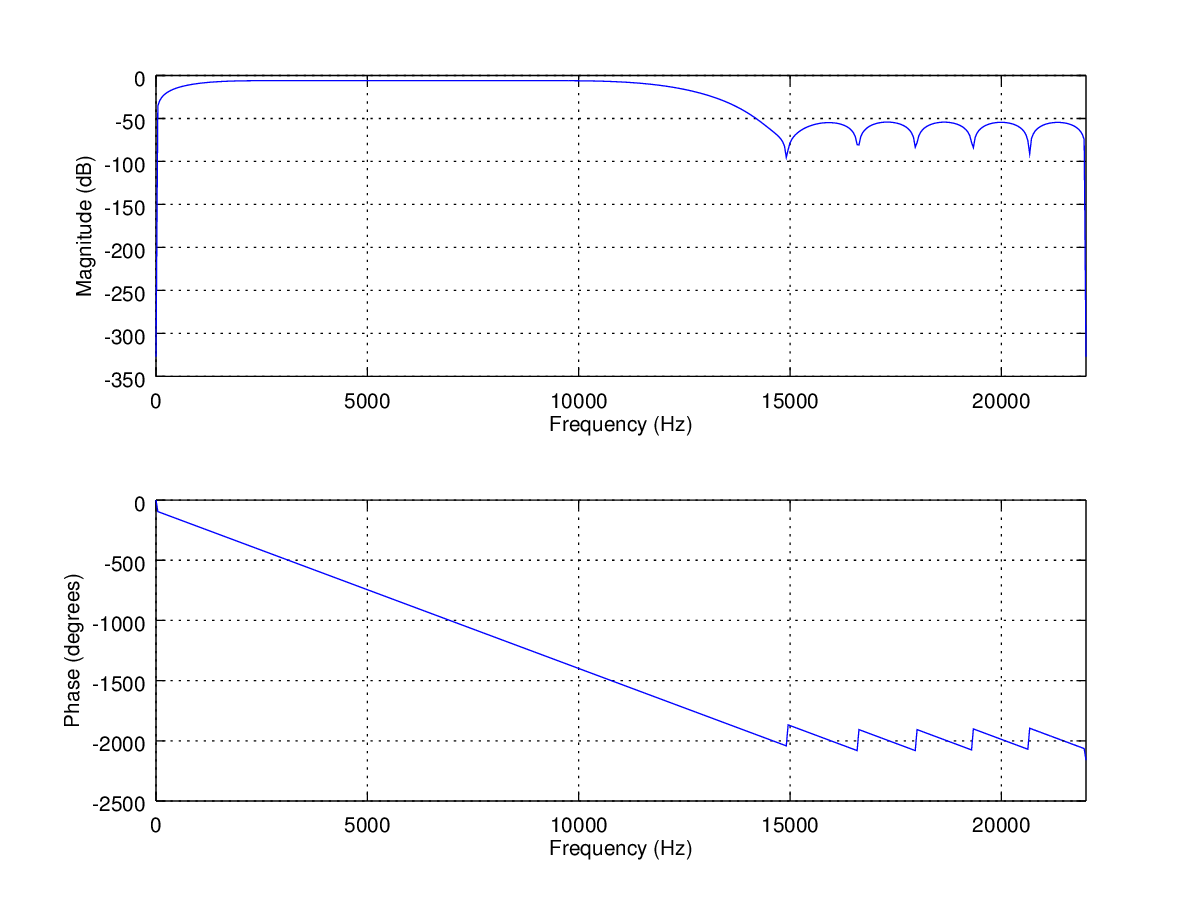
\includegraphics[scale=0.4]{../cw32_output_Hamming}
	}
	\subfloat[Okno Bartletta]{
		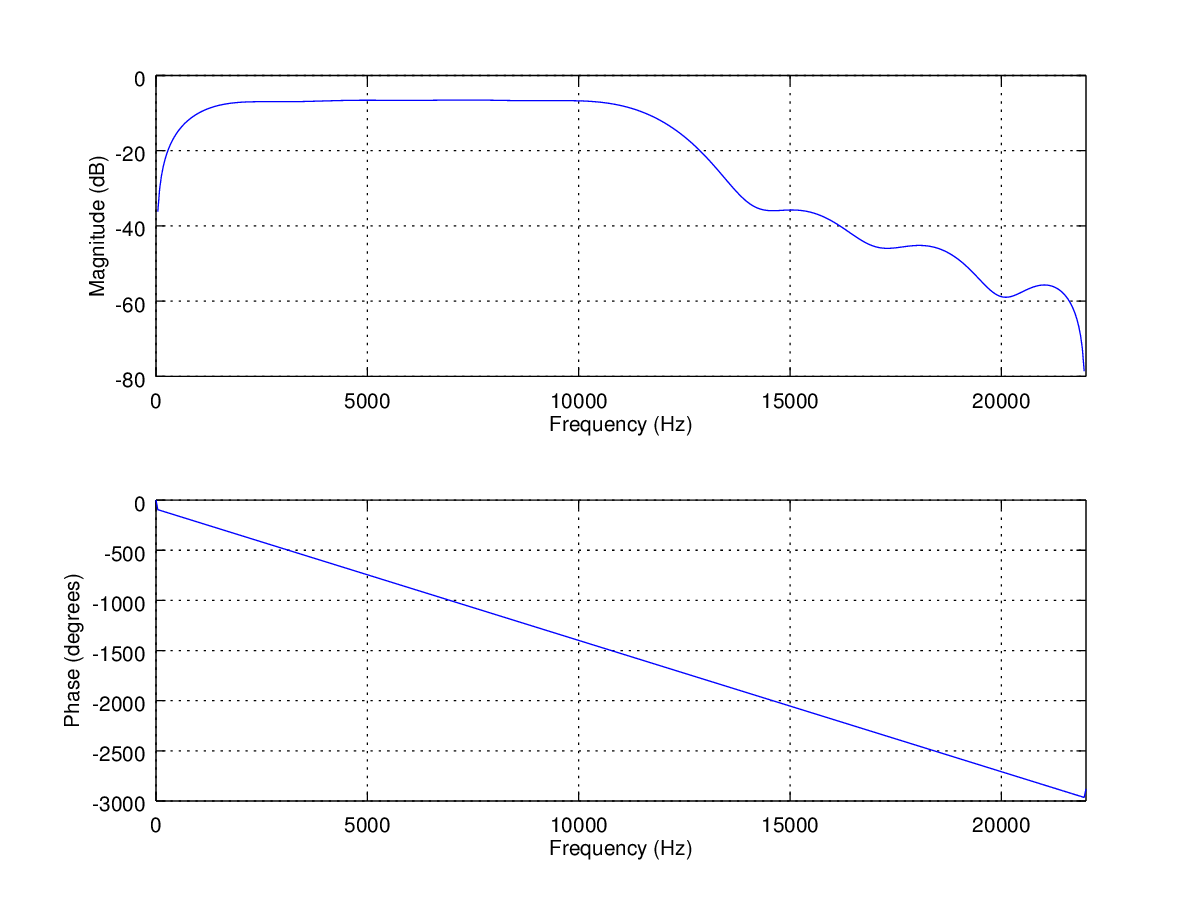
\includegraphics[scale=0.4]{../cw32_output_Bartlett}
	}
	\par
	\subfloat[okno Blackmana]{
		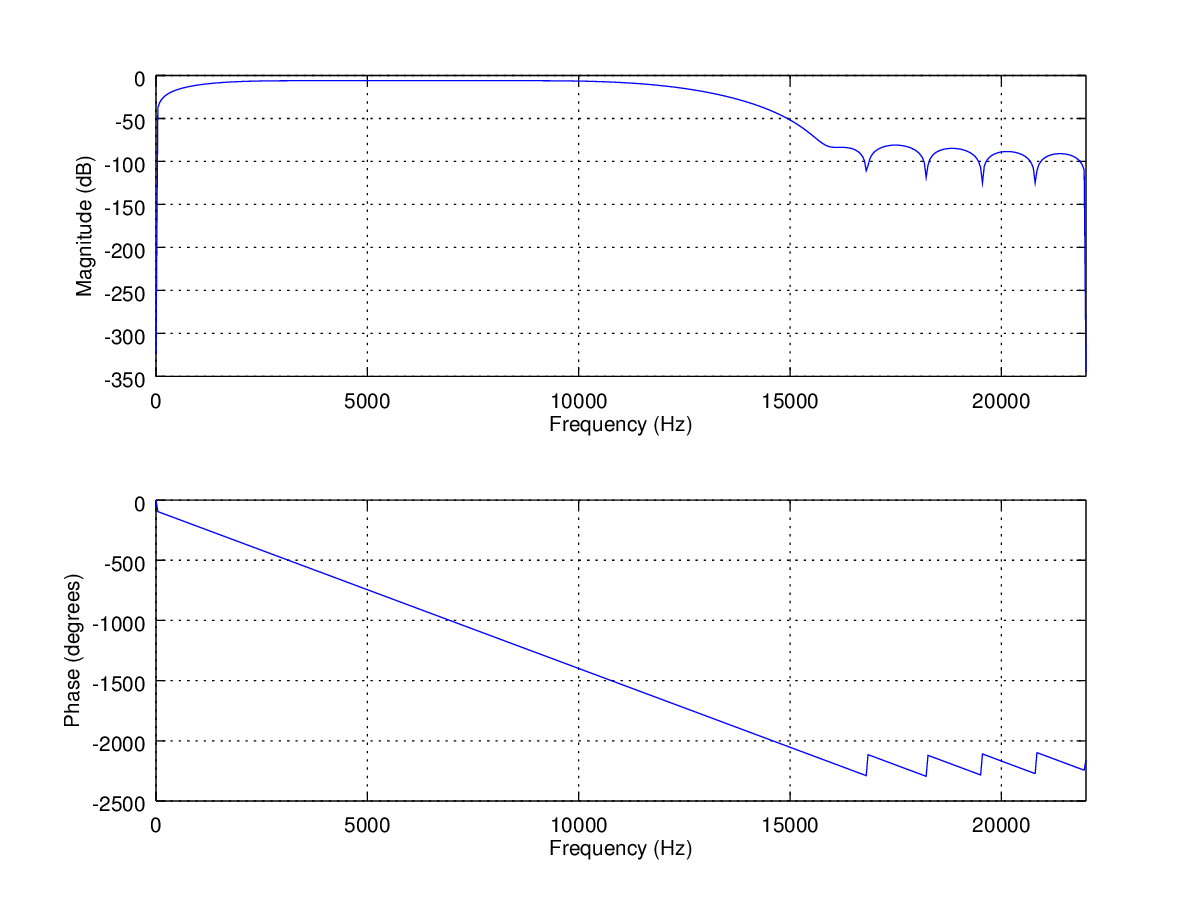
\includegraphics[scale=0.4]{../cw32_output_Blackman}
	}
	\caption{Charakterystyki projektowanych filtrów rzędu 33}
\end{figure}
Tak jak w poprzednim punkcie, Okno Bartletta charakteryzuje się najkorzystniejszą charakterystyką fazową i małą amplituda listków bocznych. Okna Hamminga i Blackmana dają za to większe tłumienie w paśmie zaporowym.
\newpage

\subsection{Filtr górnoprzepustowy}
Skrypt użyty do projektowania filtru:
{
	\tiny
	\begin{verbatim}
	n=120;
	ft = 600 /8000;
	w=blackman(n+1); %funkcja okna
	h=fir1(n, ft, 'high', w);
	H = fft(h);
	freqz(h,1,512,16000)
	\end{verbatim}
}
\begin{figure}[!h]
	\centering
	\includegraphics[scale=0.7]{../cw33_output}
	\caption{Filtr górnoprzepustowy}
\end{figure}
Powyższy filtr został wykonany w Matlabie. Poprzednie zadania wykonywane były w Octave. Zostałem zmuszony do przesiadki przez słabe wsparcie Octave dla DSP.
\newpage

\subsection{Filtr schodkowy dolnoprzepustowy}
\begin{figure}[!h]
	\centering
	\includegraphics[scale=0.5]{../cw34_polecenie}
	\caption{Zadany kształt charakterystyki filtru}
\end{figure}
Skrypt użyty do projektowania filtru:
{
	\tiny
	\begin{verbatim}
	n=200;
	fs=48000;
	ft1 = 100*(2/fs);
	ft2 = 16000*(2/fs);
	w=bartlett(n+1);
	h1=impz(fir1(n, ft1, 'low', w));
	h2=impz(fir1(n, ft2, 'low', w));
	h=(h1+h2)/2;
	freqz(h)
	\end{verbatim}
}
\begin{figure}[!h]
	\centering
	\includegraphics[scale=0.7]{../cw34_output}
	\caption{Charakterystyka zaprojektowanego filtru}
\end{figure}
Aby sprostać wymaganiom zadania zwiększyłem rząd filtru do 200.
\newpage

\section{Filtry NOI}


\end{document}